\documentclass[12pt, letterpaper, oneside]{book}
\usepackage[spanish,es-tabla]{babel}
\usepackage[utf8x]{inputenc}
\usepackage{microtype}
\usepackage{emptypage}
\usepackage{usmtesis}
\usepackage{url}
\usepackage{caption}
\usepackage{amsmath}
\usepackage{listings}
\usepackage{float}
%\usepackage{graphicx}
\usepackage{subcaption}
\usepackage{hyperref}
\usepackage{amsfonts}
\usepackage[]{tocbibind}
\usepackage{algorithm}
\usepackage[noend]{algpseudocode}
\usepackage{subcaption}
\usepackage[htt]{hyphenat}
\usepackage{listings}
\usepackage{listings-golang}
\usepackage[pdftex,dvipsnames]{xcolor}  % Coloured text etc.
\colorlet{punct}{red!60!black}
\definecolor{background}{HTML}{FFFFFF}
\definecolor{delim}{RGB}{20,105,176}
\colorlet{numb}{magenta!60!black}


\lstset{
  language=bash,
  frame=top,frame=bottom,
  basicstyle=\small\normalfont\sffamily,    % the size of the fonts that are used for the code
  stepnumber=1,                           % the step between two line-numbers. If it is 1 each line will be numbered
  numbersep=10pt,                         % how far the line-numbers are from the code
  tabsize=2,                              % tab size in blank spaces
  extendedchars=true,                     %
  breaklines=true,                        % sets automatic line breaking
  captionpos=t,                           % sets the caption-position to top
  mathescape=true,
  stringstyle=\color{white}\ttfamily, % Farbe der String
  showspaces=false,           % Leerzeichen anzeigen ?
  showtabs=false,             % Tabs anzeigen ?
  xleftmargin=17pt,
  framexleftmargin=17pt,
  framexrightmargin=17pt,
  framexbottommargin=5pt,
  framextopmargin=5pt,
  numbers=left,
  showstringspaces=false      % Leerzeichen in Strings anzeigen ?
}



\lstdefinelanguage{json}{
    basicstyle=\normalfont\ttfamily,
    numbers=left,
    numberstyle=\scriptsize,
    stepnumber=1,
    numbersep=8pt,
    showstringspaces=false,
    breaklines=true,
    frame=lines,
    backgroundcolor=\color{background},
    literate=
     *{0}{{{\color{numb}0}}}{1}
      {1}{{{\color{numb}1}}}{1}
      {2}{{{\color{numb}2}}}{1}
      {3}{{{\color{numb}3}}}{1}
      {4}{{{\color{numb}4}}}{1}
      {5}{{{\color{numb}5}}}{1}
      {6}{{{\color{numb}6}}}{1}
      {7}{{{\color{numb}7}}}{1}
      {8}{{{\color{numb}8}}}{1}
      {9}{{{\color{numb}9}}}{1}
      {:}{{{\color{punct}{:}}}}{1}
      {,}{{{\color{punct}{,}}}}{1}
      {\{}{{{\color{delim}{\{}}}}{1}
      {\}}{{{\color{delim}{\}}}}}{1}
      {[}{{{\color{delim}{[}}}}{1}
      {]}{{{\color{delim}{]}}}}{1},
}


\makeatother
%
\RequirePackage{fancyhdr}
\newcommand{\hsp}[1][20]{\hspace{#1pt}}
\fancyhf{}
\fancypagestyle{plain}{%
	\fancyhf{} 
	\fancyhead[L]{\scriptsize \rightmark}
	\fancyhead[R]{\scriptsize \leftmark}
	\fancyfoot[R]{\bfseries \thepage}
	\fancyfoot[L]{Departamento de Informática. UTFSM.}
	\renewcommand{\headrulewidth}{0.1pt}
	\renewcommand{\footrulewidth}{0.1pt}
}
%\setlength{\footheight}{110pt} 
\usepackage{xargs}                      % Use more than one optional parameter in a new commands
\usepackage[colorinlistoftodos,prependcaption]{todonotes}

%macros
\renewcommand{\tt}[1]{\texttt{#1}}
\renewcommand{\it}[1]{\textit{#1}}
\renewcommand{\bf}[1]{\textbf{#1}}
\newcommand{\etal}{\emph{et al.}}
\newcommand{\get}{$\gets$\,\,}
\newcommand{\ra}{$\rightarrow\,\,$}
\newcommand{\la}{$\leftarrow\,\,$}

\floatname{algorithm}{Algoritmo}
\renewcommand{\listalgorithmname}{Índice de algoritmos}
\renewcommand{\algorithmicrequire}{\textbf{Input:}}
\renewcommand{\algorithmicensure}{\textbf{Output:}}

\author{Maximiliano Federico Osorio Bañados}
\profguia{Carlos Buil-Aranda}
\profcorr{Marcelo Mendoza}
\profext{Daniel Garijo}
\magister
\university{Universidad Técnica Federico Santa María}
\title{REPRODUCIBILITY OF COMPUTATIONAL ENVIRONMENTS FOR SCIENTIFIC EXPERIMENTS USING-CONTAINER-BASED VIRTUALIZATION}




\setcounter{tocdepth}{1}

\begin{document}
\frontmatter
\thispagestyle{empty}
%!TEX root = main.tex

\begin{center}
  \begin{spacing}{1}
    {\large UNIVERSIDAD TÉCNICA FEDERICO SANTA MARÍA}\\
    DEPARTAMENTO DE INFORMÁTICA\\
    VALPARAÍSO - CHILE
  \end{spacing}

  \vspace{12mm}
  
\includegraphics[height=50mm]{figures/utfsm.pdf}
  \vspace{15mm}

  \begin{spacing}{1.5} 
    \textbf{\large REPRODUCIBILITY OF COMPUTATIONAL ENVIRONMENTS FOR SCIENTIFIC EXPERIMENTS USING-CONTAINER-BASED VIRTUALIZATION
}\\
  \end{spacing}

  \vspace{20mm}
  \textbf{\large MAXIMILIANO FEDERICO OSORIO BAÑADOS}
  \vspace{12mm}

  \begin{spacing}{1.25} 
    TESIS PARA OPTAR LA GRADO DE\\
    MAGÍSTER EN CIENCIAS DE LA INGENIERÍA INFORMÁTICA
  \end{spacing}

  \vfill
  \large DICIEMBRE 2018
\end{center}

\newpage

%debug
%\layout
%\newpage

%% Hack para el abstract corregir si se puede.
%\chapter*{ }
%\vspace{-3cm}
%\section*{Abstact} \chaptermark{Abstract}
%\section*{Resumen}
	\signaturepage

% The "Funny Quote Page"
\pagestyle{empty}  % No headers or footers for the following pages

\null
\vfill\vfill
\begin{flushright}
\textit{A Martín,\\por tratarme como a la mejor de tus putas.}
\end{flushright}

\vfill\vfill\vfill
\null
\clearpage 



\section*{Resumen}

La reproducibilidad experimental es la capacidad de volver a ejecutar un experimento con o sin la introducción de cambios en él y que los resultados sean consistentes con los originales. 
Para permitir la reproducibilidad, la comunidad científica ha animado a los investigadores a conservar las descripciones de estos experimentos. 
Sin embargo, el trabajo en la descripción de la infraestructura no ha resuelto de forma completa.

En este trabajo proponemos un sistema para describir automáticamente los entornos computacionales utilizados en los experimentos computacionales. 
Para ello, proponemos utilizar la virtualización basada en contenedores para distribuir los experimentos a través de imágenes de software y un sistema de anotación que permita describir estas imágenes de software. 
Las imágenes son una versión mínima de un sistema operativo (contenedor) que permite el despliegue de múltiples paquetes de software aislados dentro de él. 
Proponemos el uso de Contenedores Docker para la conservación del entorno científico y un framework para capturar el valioso conocimiento sobre los recursos de un experimento computacional que se ejecuta en un contenedor Docker.
Como resultado, nos enfrentamos al desafío lógico y físico de la conservación. 
 \newpage
\section*{Abstract}
% 
Experiment reproducibility is the ability to re-run an experiment with or without introducing changes to it and getting results that are consistent with the original ones. 
To allow reproducibility, the scientific community encourages researchers to publish descriptions of the these experiments. 
However, the recommendations for obtaining a description of the infrastructure has not resolved completely.
In this paper we propose a system to automatically describe computational environments used in in-silico experiments. We propose to use container-based virtualization for distributing software experiments throughout software images and an annotation system that will allow to describe these software images. The images are a minimal version of an OS (container) that allow the deployment of multiple isolated software packages within it. 
We propose the usage of Docker for the conservation of the scientific environment and a framework to capture the valuable knowledge about the resources of a computational experiment running on a Docker Container. As a result, we are facing the logical and physical conservation challenge. 
\begin{spacing}{1}
  \tableofcontents \chaptermark{Tabla de contenidos}
  \listoffigures
  \listoftables
  %\listofalgorithms\addcontentsline{toc}{chapter}{\bf{\listalgorithmname}}
\end{spacing}

% ******************************** Main Matter *********************************
\mainmatter

% ********************************** Preamble **********************************
% ************************** Thesis Acknowledgements **************************

\section*{Agradecimientos}

Deseo agradecer a cada una de las personas que han aportado en mi desarrollo durante los años del magister. A los nuevos amigos, a los viejos, a mi familia y a mi compañera.

Primero, deseo agradecerle a mi amigo y mentor: Jonathan. Amigo: usted me enseñó muchas cosas de Linux: de cómo darle cariño a los servidores y cómo hacer las cosas bien. 
Por ello, le agradezco tremendamente. 
Sin embargo, usted me enseño algo más importante: que los amigos y los seres queridos son lo más importante. Gracias amigazo, ánimo haciendo a Chile un lugar mejor.\\
Amigo Jesús, ya lo veo poco y nos veremos menos. Gracias por las conversaciones y vinitos compartidos, recuerde que su felicidad está primero.
Al ``El amigo Sergio", como usted bien sabe: ``el trabajo es la peor tortura". Sin embargo, ir a trabajar con usted era un chiste (gracias). 
Fabián, gracias por enseñarme tus tips de batallas y historias de vida, me aportaron para crecer. 
Juan Pablo, me caí bien y no se porqué... Bueno, trabajar contigo fue entretenido, gracias por aportar en mi desarrollo profesional y personal.\\
Amigo Dave, gracias por invitarme a tu depa con el Jonathan, por recordarme que todavía tengo pasión por aprender. Algún día tomaré su oferta.\\
Carlos Buil, Carlitos. Primero, gracias por el consejo de botar mi tesis anterior, gracias por no ser un profesor egoísta que busca exprimir a sus estudiantes en beneficio propio\footnote{Bonnaire tu no, gracias por apoyarme en botar la tesis}. Sino para ayudarlos. Gracias por estar seguro que DockerPedia podría ser un trabajo exitoso, por la buena onda para trabajar, cuando te moviste para que la tesis tuviera platita y por presentarme a Dani Garijo.
Dani, gracias por tus gestiones para la posición en ISI y por ser mi profesor externo; tener un experto en el tema es un honor para mí. Esperemos que todo resulte bien en ISI.

Andres, lo primero es lo primero: Felipe Avello, cuantas risas viendo a Avello. De hecho, lo voy a ver ahora... sin la avello-terapia, la vida no es lo mismo. Gracias por las conversaciones en el departamento y esas voladas brigidas que me ayudaron a tomar buenas decisiones. Y por supuesto, gracias por traer la música a mi cabeza.
Loco Peréz, gracias por todos esos combos de pizza más los ingredientes secretos, que buenos momentos, el sillón aún te recuerda.

Hernan, primero gracias por tu ayuda en DockerPedia. Conocer gente como tú es un agrado y es impagable, gracias por abrir mi mente. Sos un grande.

Camilo, Camilito. Vos me caí muy bien, es que eres un amor, gracias por aguantar todas las tonteras que hice en: el lab, calle, universidad, transporte público, ruka, café, bares y en telegram.
Leito, gracias por esos rukazos compartidos, por creer que DockerPedia era un buen humito, y por darme el curso de Sistemas Operativos (el alcohol sale dinero).

Amigo Gonzalo, claramente faltaron más días en Linets para combatir contra el empresariado. Espero que esos PES épicos se repitan. Disculpe por el mar de preguntas.
Diego, qué buenos momentos tuvimos vacilando en el departamento. Usted es un amigazo, de esos buenos, que uno debe mantener.
Amigo Marcelo, usted es un ser del luz y un excelente amigo, qué buenas conversaciones nos mandamos tratando de entender todo. Amigo, gracias por las palabras que han aportado en mi vida.\\
\texttt{
Martin?
Why is it so hard
To make it in Sapito?
I try so hard
To make it in Sapito.}
Compartir el departamento fue un chiste: Las copas rotas al ritmo de One My Turns, esas peleas de pantuflas, su batalla de correas, esas peleas con cuchillo y raquetas eléctricas, o cuando ibamos a dar clases de PES al 801. 
Eres un tremendo amigo, gracias por esos muy recuerdos. Espero que sigas ayudando a que Don Arturo tenga los precios más bajos. Espero que disfrutes con la Fabiola. Y dile a Torres que pare su vacilé.\\
Tomi (pero Verrati), Cristian (faltan sus pes), Ariel (que grandes cumbias), Jorgito (ratón, ratón), Axel (fuiste parte de la venganza de Gemoya, perdono pero no olvido), Germán (tremenda persona que me faltó conocer más), Carlangas (nos vemos en segunda), Roberto (que agrado escuchar su risa), pibarra (liberen a pibarra, ya pos Torres, el pan de pascua), amigo Fabian (que buena persona, menos mal que no hice ejercicio con usted), Ignacio (que buenas conservaciones de pasillo sobre el veganismo que compartimos), Eduardo (gracias por la vez que salimos correr y compartir cafecito), Sazo (esos pes con O'Higgins en Santiago y las copas). Daniela (por esa conversación mirando el santiago nublado), Dossow (por prestarme el cable el día que rompí el universo), Esteban (por esas cervezas y la idea de ir a Buenos Aires), Tamara y Felipe (gracias por recibirnos en Santiago y compartir su vida).
Cabres en general, ustedes notaron mi cambio y los resultados. Cada uno de ustedes fue un aporte en ese crecimiento. Gracias.\\
Amigos de CSRG: madiaz, Vicente, Rodrigo, Daniel San Martin (fuerza en su doctorado, busque muchos consejos), cjaregui y maray gracias por las risas y aguantar todas las temas que ponía a todo volumen en el lab.
Amigo Francisco Casas, le hago una nota especial porque los seres de luz siempre lo merecen. Cuídese mucho y disfrute su vida.\\
Antes de agradecer a mi familia, quiero agradecer a Marcelo Bielsa: Gracias por su trabajo y sus enseñanzas, gracias por permitir que mi padre disfrutará el juego de Chile.
También a Gilmour, Waters, Mason, Wright y Syd por explotar mi cabeza de ideas.

Hermana, gracias por querer lo mejor para mí, por emocionarte cuando les conté que ahora estoy muy feliz. Gracias hermanita.
Toño, gracias por acompañar a mi hermana, por acompañar y ayudar a mis padres y abuela; por ayudar en esas tareas de hijo y nieto. Gracias.\\
Hermano, gracias por tu consejo que no debía seguir en Chile y querer más. Por apoyarme en la decisión de renunciar e ingresar en el peor magister. Quiero decirte que estoy orgulloso de tu perseverancia y espero verte cuando corras tu Ironman. Pese a que no somos esos hermanos cercanos porque somos giles, sé lo que me quieres. Gracias por eso.
Kathy, primero gracias por mostrarme a Jorge Drexler, durante estos años fue y es mi banda sonora. Segundo, por creer en mis talentos. Tercero, por cuidar a tu hermano. Sigue con lo que quieras hacer.
Papá y Mama, sin su esfuerzo, probablemente yo hubiese sido un niño sin oportunidades. Gracias por cubrir lo que El Estado (si todos nosotros) debemos asegurar para todos. 
Gracias por entregar sus mejores años luchando y sufriendo por nosotros. Sin ustedes, esto no es posible. Los quiero.
Meche, estas palabras son duras, te he olvidado y tú fuiste de las personas que siempre me cuido y sacrifico muchas cosas por mí. Gracias, te quiero.
Pita, espero que mi padre le esté leyendo esto. Disculpe por no estar más con usted y dejarla sola. Usted es una mujer muy fuerte que hizo muchas cosas por mi padre y por nosotros. Descanse mucho, la queremos.

Pamela, te conocí cuando ya no buscaba a alguien, llegaste cuando me iba a Santiago. 
Y hiciste que abriera mis miedos, mi mente y mi calendario, y te volviste mi compañera y amiga, y me apoyaste en cada una de mis decisiones, me dejaste correr y gritar todo lo quisiera, me dejaste soñar y errar todo lo que quisiera, me permitiste crecer todo lo que quisiera, me enseñaste, me cuidaste y me amaste. 
Por eso, no quiero parar jamás de mirar tu carita de curadita, tan bonita (Julio Piña, 2015). 
Te amo Pamela. Se feliz (como \textbf{tú} quieras). 


Todos: ``sean felices, que estamos vivos por milagro, y nada vale más que la vida, y que es nuestro deber biológico, y por encima de todas las cosas: Respetar la vida e impulsarla" (Mujica, 2013).




\chapter{Introducción}
\label{Chapter1} 
\newcommand{\keyword}[1]{\textbf{#1}}
\newcommand{\tabhead}[1]{\textbf{#1}}
\newcommand{\code}[1]{\texttt{#1}}
\newcommand{\file}[1]{\texttt{\bfseries#1}}
\newcommand{\option}[1]{\texttt{\itshape#1}}
\improvement{cita} 
Investigadores han argumentado sobre la importancia de poder reproducir experimentos científicos debido a la necesidad de corroborar los resultados o de contribuir en el mismo trabajo.   \todo[inline]{dónde? cita}
Sin embargo, el proceso de reproducibilidad puede ser tan complejo y costoso que ha sido referido como una tarea del tipo forense \cite{baggerly2009deriving}.
De hecho, estudios controversiales y escándalos han expuesto la necesidad de mejorar los procesos de reproducibilidad de las investigaciones. Algunos ejemplos son: casos clínicos \cite{ioannidis2009repeatability}, sondeos del área de psicología \cite{open2015estimating} o estudios en área de la computación \cite{baggerly2009deriving}.\todo[inline]{utilizas frases muy cortas, esto no es inglés}
La reproducibilidad del experimento es la capacidad de volver a ejecutar un experimento con o sin la introducción de cambios en él y la obtención de resultados que sean consistentes con los originales.
La introducción de cambios permite evaluar diferentes características de ese experimento ya que los investigadores pueden modificarlo gradualmente, mejorando y re-orientando los métodos y condiciones experimentales~\cite{stodden2010reproducible}.\todo[inline]{esto tiene que ir al principio de la sección, empiezas hablando de reproducibilidad sin decir lo que es.}
Para permitir la reproducibilidad del experimento es necesario proporcionar suficiente información sobre él mismo, permitiendo comprenderlo, evaluarlo y volver a construirlo. 
Normalmente, los experimentos se describen en flujos de trabajo científicos o \emph{workflows} (representaciones que permiten gestionar cálculos a gran escala) que puede ser ejecutados en sistemas informáticos distribuidos.
%Aparece el problema de la conservación de los experimentos
Para permitir la reproducibilidad de estos workflows científicos es necesario, en primer lugar, abordar un problema de conservación del experimento.
La conservación es un acto de proporcionar información compresible que describa el contexto original del experimento y es por ello que los workflows experimentales necesitan garantizar que exista suficiente información sobre los experimentos para que sea posible construirlos nuevamente por un tercero, replicando sus resultados sin ninguna información adicional del autor original ~\cite{garijo2013quantifying}.
%Cual es la conversación que se hace ahora
Para alcanzar la conservación, la comunidad se ha enfocado en la conservación de las ejecuciones de workflow conservando los datos, código y la descripción, pero dejando de lado la infraestructura subyacente (e.g, recursos computacionales y componentes de software).
Existe enfoques que se han enfocado en conservar el ambiente computacional de un experimento como WICUS~\cite{santana2017reproducibility} que propone vocabularios semánticos para la conservación o el proyecto TIMBUS~\footnote{\url{http://www.timbusproject.net/}}~\cite{dappert2013describing} que describe los procesos de negocios y el software y el hardware subyacente.

%Hablamos los tipos de conservación que existe
Los autores en~\cite{santana2017reproducibility} identificaron dos enfoques para conservar el ambiente computacional de un experimento científico: la conservación física, en la que los objetos de investigación dentro del experimento se conservan en un entorno virtual (e.g., máquinas virtuales); y la conservación lógica, en la que se describen las principales capacidades de los recursos del ambiente computacional utilizando vocabularios semánticos para que el investigador pueda reproducir un entorno equivalente.
Para ello, definieron un proceso para documentar la aplicación de workflow, su sistema de gestión relacionado y las dependencias de ambos.
Sin embargo, este proceso es manual, dejando un trabajo complejo para los científicos. 
Además, al igual que la mayoría de los trabajos dejan fuera del alcance la conservación física del entorno computacional del workflow debido a los costos de infraestructura que mantenga los datos, restricciones políticas de las organizaciones a cargo y procesos de decaimiento.\todo[inline]{no se entiende esta frase}
Sin embargo, la conservación física simplifica la ejecución del experimento a cargo de nuevo investigador. Dado que evita el proceso de reconstrucción del ambiente que es una tarea compleja.
El problema de reproducibilidad no sólo sucede en la comunidad científica. Compañías tecnológicas también enfrenta problemas similares cuando ellos desean distribuir cualquier producto de software a múltiples servidores o plataformas.
Para resolver esto, las compañías utilizan la virtualización. Esta tecnología se refiere a una característica del Sistema Operativo (SO) en la que el kernel del SO permite la existencia de múltiples instancias aisladas de espacio de usuario llamadas máquinas virtuales o contenedores.
Una de las tecnologías de virtualización más populares en la industria es Docker\footnote{\url{https://www.docker.com/}}, que implementa la virtualización de software mediante la creación de versiones mínimas de un sistema operativo base (un contenedor).
Docker Containers pueden ser vistos como máquinas virtuales ligeras que permiten el ensamblaje de un entorno computacional, incluyendo todas las dependencias necesarias, como bibliotecas, configuración, código y datos, entre otros.
%need
Para reproducir experimentos científicos computacionales de otros investigadores, es obligatorio permitir que los científicos compartan estos experimentos o conservar su ambiente computación con el objetivo de reproducir el ambiente computacional  (el mismo o muy similar).
De esta manera, un científico tendrá garantías de que el experimento se está ejecutando en el mismo entorno o similar en comparación al entorno original.
Por lo tanto, se necesita un procedimiento que garantice ambos requisitos: preservar los entornos tanto lógicos como físicos para volver a ejecutar los flujos de trabajo de datos con garantías de reproducibilidad.
Para permitir la conservación es necesario, proporcionar una manera de describir el entorno computacional en el que se ejecutó el experimento. 
La conservación lógica permite describir el entorno computacional en el que se ejecutó el experimento, por lo tanto los investigadores pueden conocer los componentes de software y al volver a construir el ambiente computacional del experimento y conocer cuáles los cambios que sean producido a nivel de los recurso.
Considerando lo anterior, se propone una solución para mejorar la solución de conservación física y lógica mediante el uso de contenedores.\todo[inline]{solo contenedores?}\todo[inline]{aquí deberías decir cuál es tu hipótesis}
Se propone en primer lugar utilizar las imágenes Docker como medio para preservar el entorno físico de un experimento. Se utilizan contenedores ya que son ligeros, de fácil adopción y lo que es más importante, son más fáciles de describir automáticamente, por lo que se mejora el proceso de documentación de los workflows científicos.
Con Docker, los usuarios pueden distribuir estos entornos computacionales a través de imágenes de software utilizando un repositorio público llamado DockerHub. Por lo tanto, se alcanza la conservación física descansado en los repositorios.
Con el fin de lograr una conservación lógica, se construye un sistema de anotador para las imágenes Docker que describe el sistema de gestión del workflow y las dependencias asociados. De esta manera, se pretende abordar la conservación lógica.
Para validar la solución se reproducen cuatros experimentos computacionales diferentes. Estos experimentos abarcan diferentes sistemas de workflows, lenguajes y configuraciones, lo que demuestra que el enfoque es genérico y puede aplicarse a múltiples experimentos computacionales.
Se construyen los ambientes computacionales de estos experimentos, se describen lógicamente, se utiliza estas descripciones para la resolución de problemas de ejecución y se reproduce el ambiente computacional en base a las descripciones lógicas que se obtuvieron anteriormente.
Para validar el enfoque, se comparan los valores o estructuras de los resultados de los experimentos y registro de eventos de información o errores del sistema de workflow.
\chapter{Estado del arte}\label{Chapter2} 
\section{Conservación de procedimiento científicos}

Distintas áreas de la ciencia han adoptado técnicas y herramientas para conservar el procedimiento. Por ejemplo, investigadores en bio-informática ha incorporado los workflows para distintos análisis:  Doblamiento de proteínas \cite{craddock2006science}, secuencias de DNA y RNA \cite{blankenberg2010galaxy,giardine2005galaxy} y la detección de ondas gravitacionales \cite{deelman2004pegasus}.
Los workflows científicos son métodos que permiten representar un conjunto de pasos computacionales. Estos pasos pueden ser la obtención de los datos de entrada, transformaciones o generación de los resultados.
La representación de los workflow se construye en un lenguaje abstracto para simplificar la complejidad. El conjunto de pasos se pueden representar como grafos sin ciclos y dirigidos, donde cada paso computacional es representado por un nodo y las dependencias entre los pasos son representado por los arcos.
El uso de sistemas de manejo de workflows científicos \textit{Scientific Workflow management Systems (WMS)} permiten diseñar abstractamente, ejecutar y compartir el procedimiento científicos. 

Dado que los workflows formalmente describen la secuencia de tareas computacionales y administración de datos, es fácil encontrar el camino de los datos producidos.
Un científico podría ver el workflow y los datos, seguir los pasos y llegar al mismo resultado. En otras palabras, la representación del workflow facilita la creación y administración de la computación y además construye una base en la cual los resultados pueden ser validados y compartidos.


\subsection{Sistemas de administración de workflows}

Cómo se menciono anteriormente, los workflows científicos permiten a los usuarios expresar fácilmente tareas computacionales de varios pasos, por ejemplo, recuperar datos de un instrumento o una base de datos, dar un formato a los datos y ejecutar un análisis. 
Un workflow científico describe las dependencias entre las tareas y la mayoría de los WMSs utiliza la descripción de un gráfico acíclico dirigido (DAG), donde los nodos son tareas y los bordes denotan las dependencias de las tareas.
Una propiedad que define un workflow científico es que gestiona el flujo de datos. Es por ello, que las tareas en un  workflow científico varían ampliamente según las necesidades del autor, los tipos pueden ser tanto como tareas cortas en serie o tareas paralelas muy grandes (e.g, utilizando Message Passing Interface - MPI) rodeadas de un gran número de pequeñas tareas en serie utilizadas para el pre y post procesamiento.
La interpretación y ejecución de los workflows son manejados por un sistema de manejo de workflows (WMS) que administra la ejecución de la aplicación en la infraestructura. 
Un WMS puede ser considerado como una capa intermedia necesaria para la abstracción y orquestación de procedimiento científico. A continuación se describen algunos de los WMSs más populares.

\subsection{Galaxy}	
Galaxy \cite{goecks2010galaxy} es un sistema de gestión de almacenes basado en la web que tiene como objetivo llevar las capacidades de análisis de datos computacionales a usuarios no expertos en el campo de las ciencias biológicas. Los principales objetivos del marco de trabajo de Galaxy son la accesibilidad a las capacidades computacionales biológicas y la reproducibilidad del resultado del análisis mediante el seguimiento de la información relacionada con cada paso del proceso. 

\subsection{Taverna}	
Taverna \cite{DBLP:journals/bioinformatics/OinnAFMSGCGPWL04} es un WMS basado en servicios web, ya que todos los componentes del flujo de trabajo deben implementarse cómo servicios web (ya sea localmente o utilizando un servicio remoto disponible). 
Taverna permite a un científico que tiene una experiencia limitada en informática, recursos técnicos y soporte limitados, construir análisis altamente complejos sobre datos y recursos computacionales que son tanto públicos como privados, utilizando cualquier sistema operativo.
Además, Taverna provee integraciones con myExperiment~\cite{goble2010myexperiment} y BioCatalogue~\cite{bhagat2010biocatalogue} y provee servicios para ejecutar código Java local, uso de lenguaje R \footnote{\url{https://www.r-project.org/}} , scripts XPath o servicios de importación de hojas de cálculo.

\subsection{Pegasus}
Pegasus\cite{deelman2004pegasus} abarca un conjunto de tecnologías que ayudan a que las aplicaciones basadas en workflow se ejecuten en diferentes entornos, incluyendo escritorios, clusters de campus, grillas y nubes. Pegasus tiende un puente entre el dominio científico y el entorno de ejecución mediante la asignación automática de descripciones de workflow de alto nivel a recursos distribuidos. 
Siendo capaz gestionar flujos de trabajo compuestos por millones de tareas, registrando datos sobre la ejecución y resultados intermedios.
En Pegasus, los flujos de trabajo se describen como flujos de trabajo abstractos, que no contienen información de recursos, o las ubicaciones físicas de datos y ejecutables.

\subsection{WINGS}  
 
WINGS \cite{DBLP:journals/expert/GilRKGGMD11} es un sistema de workflow semántico que ayuda a los científicos en el diseño de experimentos computacionales.
La diferenciación de WINGS respecto a otros WMSs es que incorporan restricciones semánticas sobre conjuntos de datos y componentes de flujo de trabajo, a partir de esas restricciones éstos se crean y validan para generar los resultados.  
WINGS puede considerarse como una herramienta de diseño de alto nivel y orientada a los dominios, cuyos workflows pueden ejecutarse posteriormente en diferentes motores de WMSs, como Pegasus~\cite{deelman2004pegasus} o Apache OODT \footnote{\url{http://oodt.apache.org/}}.

\subsection{dispel4py}
dispel4py \cite{DBLP:conf/eScience/FilgueiraKAKSS15}  es una biblioteca Python para describir flujos de trabajo. 
 Describe flujos de trabajo abstractos para aplicaciones intensivas en datos, que luego se traducen y ejecutan en plataformas distribuidas (por ejemplo, Apache Storm, clusters MPI, etc.).
Uno de los objetivos es que los usuarios se centren en sus métodos científicos, evitando que se distraigan en los detalles y manteniendo la flexibilidad sobre la infraestructura informática que utilizan. 


\section{Conservación de equipamiento}
Comúnmente en otras disciplinas que realizan estudios \emph{in-vivo}, el equipamiento no es un problema a resolver dado que los recursos utilizados son conocidos, no-variables y estándares. Por ejemplo en la biología ó quimica, la utilización de probetas, microscopios u otros elementos físicos. 
Consecuentemente, los investigadores pueden nombrarlos e identificarlos de forma manual en los procedimientos de sus cuadernos de laboratorio. Lo que permite que otro investigador conozca cuáles fueron las herramientas utilizadas en el experimento.
Aunque existen excepciones, donde ciertos recursos son materiales que son utilizados en los procedimientos. En estos casos, los investigadores deben describir los materiales incluyendo información como marcas, composición y otros. 
Otro caso es en la astronomía, donde se utilizan recursos de alta tecnología, donde también es necesario documentar las características de hardware y configuraciones utilizadas en el proceso experimental. 
En las ciencias de la computación sucede un caso similar, dado que los recursos computacionales son una componente requerida en la ejecución del sistema. 
Es por ello, que esta comunidad no puede ser la excepción respecto a la descripción de los recursos. Por lo tanto, los autores deben documentar computadores, clusters, servicios web, componentes de software, etc., en el contexto de sus experimentos.

Diversos trabajos han estudiado el estado actual de la reproducibilidad de estudios \emph{in-silico}, en \cite{DBLP:conf/eScience/ZhaoGBKGGHRRG12} se estudia el factor de decaimiento de un conjunto workflows científicos almacenado en myExperiment \footnote{\url{https://www.myexperiment.org/home}} que fueron diseñados para el WMS Taverna \cite{DBLP:journals/bioinformatics/OinnAFMSGCGPWL04} del área de biología. Para ello, los autores utilizaron cuatro conjuntos de paquetes de workflows y clasificaron el decaimiento de los workflows en cuatro categorías: recursos de terceros volátiles, datos de ejemplos faltantes, ambiente de ejecución faltante y descripciones insuficientes sobre los workflow. El estudio muestra que casi el 80\% de workflows fallan al ser reproducidos, con un 12\% de esos fallos debido al ambiente de ejecución faltante y 50\% recursos de terceros volátiles. Estas dos últimas categorías están asociadas a la conservación del ambiente computacional del experimento.
En \cite{DBLP:conf/ipres/MatthewsCWJBS09}, los autores describen un procedimiento para preservar el software, argumentando que el software es frágil a los cambios de ambiente ya sea hardware, sistema operativo, versiones de las dependencias y configuración. Los autores afirman que el software no puede ser preservado con la metodología de sólo mantener su código binario ejecutable recomendando el empaquetamiento de software. También, introducen el concepto de adecuación de la preservación, una métrica para medir si la preservación de conjunto de funcionalidades de componente de software luego de un proceso reproducción.

De la misma manera, editoriales se ha enfocado en intentar resolver los desafíos en la publicación de trabajos científicos. Por ejemplo, Elsevier formó el \textit{Executable Paper Grand Challenge} para abordar la dificultad de reproducibilidad de los resultados en las ciencias de la computación, ellos  argumentan que los bloques vitales y necesarios de información para replicar los resultados -por ejemplo, software, código, grandes conjuntos de datos- no suelen estar disponibles en el contexto de una publicación académica. 
Es por ello que \textit{Executable Paper Grand Challenge} creó una oportunidad para que los científicos diseñen soluciones que capturen esta información y proporcionen una plataforma para que estos datos puedan ser verificados y manipulados. 
En 2011, \cite{DBLP:journals/procedia/BrammerCMW11} se argumenta que el documento de investigación en su estado actual ya no es suficiente para reproducir, validar o revisar completamente los resultados y conclusiones experimentales de un documento. Esto impide el progreso científico. 
Para remediar estas preocupaciones, presentan Paper Mâché, un nuevo sistema para crear documentos de investigación dinámicos y ejecutables. La principal novedad de Paper Mâché es el uso de máquinas virtuales, que permite a los lectores y revisores ver e interactuar fácilmente con un documento y poder reproducir los principales resultados experimentales.
En la misma línea, CernVM~\footnote{\url{https://cernvm.cern.ch/}}~\cite{buncic2010cernvm} propuso la utilización de máquinas virtuales para resolver problemas de reproducibilidad en la ciencia. CernVM es un sistema para el uso de máquina virtuales capaz de ejecutar aplicaciones físicas de los experimentos relacionados al \textit{Large Hadron Collider} (LHC) en el \textit{European Organization for Nuclear Research} (CERN). Su objetivo es proporcionar un entorno completo y portátil para desarrollar y ejecutar el análisis de datos generados por el LHC en cualquier ordenador del usuario final (portátil, de mesa), así como en la red, independientemente de las plataformas de sistemas operativos (Linux, Windows, MacOS). 
CernVM logra lo anterior haciendo so de técnicas de virtualización que permite separar los recursos de computación desde la infraestructura subyacente.

Algunos autores han expuesto la necesidad de capturar y preservar el entorno de ejecución del experimento, proporcionando herramientas para analizar y empaquetar los recursos involucrados en él.
ReproZip \cite{DBLP:conf/tapp/ChirigatiSF13} busca captar el conocimiento sobre una infraestructura e intentar reproducirla en un nuevo entorno. Esta herramienta lee los componentes de infraestructura involucrados en la ejecución (archivos, variables de entorno, etc.) y almacena esta información en una base de datos MongoDB \footnote{\url{https://www.mongodb.com/es}}. 
A continuación se recogen y empaquetan los elementos descritos. Luego, el sistema debe desempaquetar los elementos en otra máquina para reproducir el experimento. 
Sin embargo, este tipo de enfoque que empaqueta los componentes físicos de una infraestructura determinada presenta una limitación en la práctica, debido que los paquetes deben ser ejecutado en una máquina destino similar.
Otro ejemplo es TOSCA (Topology and Orchestration Specification for Cloud Applications), TOSCA es un ejemplo de las soluciones que han definido sintaxis para describir la ejecución de los ambientes computacionales. TOSCA es un lenguaje de código abierto utilizado para describir las relaciones y dependencias entre servicios y aplicaciones que residen en una plataforma de computación. TOSCA puede describir un servicio de computación en nube y sus componentes y documentar la forma en que están organizados y el proceso de orquestación necesario para utilizar o modificar dichos componentes y servicios. Esto proporciona a los administradores una forma común de gestionar aplicaciones y servicios en la nube, de modo que esas aplicaciones y servicios puedan ser portátiles a través de las diferentes plataformas de los proveedores de Cloud Computing. 
Otro esfuerzo importante relacionado a nuestro trabajo incluye la descripción de los ambientes computaciones utilizando ontologías es TIMBUS. El proyecto se focaliza en preservar procesos de negocios y su infraestructura computacional. 
Para ello, propusieron un extractor para extraer y anotar los componentes de Software y Hardware, éstas anotaciones son almacenadas según un conjunto de ontologías con el objetivo de gestionar la preservación y ejecución de los procesos de negocio. 
Sin embargo, el enfoque extractor del Proyecto Timbus no es adecuado para ser utilizado en cualquier sistema ya que aumenta la complejidad del ambiente y exige la instalación de componentes de terceros dentro del ambiente, lo cual provoca ruido. 
Además, exige ejecutar el ambiente computacional lo cual conlleva altos costos computacionales, disminución en la escalabilidad del sistema y creación de brechas de seguridad. 

En el enfoque de describir los recursos computacionales, los autores en \cite{santana2017reproducibility} identificaron dos enfoques para conservar el  ambiente computacional de un experimento científico: la conservación física, donde los objetos de investigación dentro del experimento se conservan en un entorno virtual; y la conservación lógica, donde las principales capacidades de los recursos en el entorno se describen utilizando vocabularios semánticos para permitir al investigador reproducir un entorno equivalente.
Para ello, definieron un proceso para documentar la aplicación del workflow y su sistema de gestión relacionado, así como sus dependencias.
Además, los autores propusieron \textit{The Workflow Infrastructure Conservation Using Semantics ontology} (WICUS). WICUS es una red de ontologías OWL2 (Web Ontology Language)~\cite{motik2009owl} que implementan la conceptualización de los principales dominios de una infraestructura computacional. Como: Hardware, Software, Workflow y Recursos Informáticos. 
Los autores argumentan su importancia de su trabajo debido que a que los workflows científicos requieren un conjunto de componentes de software, y los investigadores deben saber cómo desplegar esta pila de software para lograr un entorno equivalente.
Sin embargo, este proceso se realiza de forma de manual, dejando mucho trabajo a los científicos
En el trabajo, los autores no enfrentan la conservación física del entorno computacional argumentando tres motivos: (i) que los costos necesarios para almacenar los máquinas virtuales (ambiente) son muy altos, (ii) la existencia de dificultades dado a las restricciones políticas de las organizaciones a cargo y (iii)Chapters/Chapter1/chapter1.tex procesos de decaimiento del ambiente computacional en el tiempo~\cite{DBLP:journals/fgcs/DeelmanVJRCMMCS15}

Consecuentemente, la mayoría de los trabajos dejan fuera la conservación física del entorno informático del workflow. Pese a que la conservación lógica y física son deseadas para lograr la reproducibilidad del experimento.

En diversos trabajos ~\cite{DBLP:journals/bioinformatics/LeprevostGARUBV17, Beaulieu2017, Boettiger:2015:IDR:2723872.2723882, aranguren2015enhanced} se ha propuesto la utilización de Docker como un reemplazo al uso de máquinas virtuales como ambiente computacionales científicos, los trabajos argumentan que Docker presenta beneficios de portabilidad, documentación precisa de la instalación y configuración, manejo de control de versiones de las imágenes y fácil adopción por desarrolladores. 
Un ejemplo de uso de Docker para la reproducibilidad es Bio Containers \cite{DBLP:journals/bioinformatics/LeprevostGARUBV17}. Bio Containers es un framework de código abierto y orientado a la comunidad que proporciona entornos ejecutables independientes de la plataforma para el software de informática.
Bio Containers permite a los laboratorios instalar fácilmente software de bio-informática, mantener múltiples versiones del mismo software y combinar herramientas de análisis. 
Para ello, se basan en los populares proyectos de código abierto Docker~\footnote{\url{https://www.docker.com/}}, Singularity~\footnote{\url{https://www.sylabs.io/singularity/}} y rkt~\footnote{\url{https://coreos.com/rkt/}}, que permiten que el software sea instalado y ejecutado bajo un entorno aislado y controlado.
Sin embargo, en \cite{Boettiger:2015:IDR:2723872.2723882,DBLP:conf/semweb/OsorioAV18} los autores exponen que Docker no controla que paquetes instalados en las imágenes y no existe una descripción completa de los componentes de la imagen y consecuente del contenedor.
Por lo tanto, las imágenes Docker funcionan como una caja negra, lo que significa que los usuarios saben cuál es el paquete que se ejecuta dentro del contenedor pero no conocen las versiones o los otros paquetes necesarios para ejecutarlo.

Respecto a la descripción de los componentes de una imagen Docker, en \cite{Shu:2017:SSV:3029806.3029832:DockerHub:Security} analizó más de 300.000 imágenes de Docker almacenadas en el repositorio oficial de Docker. Los autores encontraron que en promedio las imágenes que contiene el Docker Hub (sistema de almacenamiento de imágenes) son más de 180 vulnerabilidades, siendo la raíz de tal cantidad de vulnerabilidades el hecho de que muchas imágenes no han sido actualizadas en varios días y que muchas de estas vulnerabilidades se propagan de imágenes de padres a hijos. Los autores encontraron correlaciones entre las imágenes más influyentes y los paquetes vulnerables mejor clasificados, lo que sugiere que la fuente de esa cantidad de vulnerabilidades era probablemente el resultado de la propagación de un pequeño número de imágenes populares (debido a la falta de actualización de las imágenes principales). Los autores utilizaron el software Clair \footnote{\url{https://github.com/coreos/clair}} de la empresa CoreOS\footnote{\url{https://coreos.com/}}. 
En términos de ingeniería ontológica, los autores en~\cite{huo2015smart} presentan la ontología Smart contenedor que extiende DOLCE~\cite{gangemi2002sweetening} y modela Docker en términos de sus interacciones para desplegar imágenes. Otro trabajo relacionado, ~\cite{tommasini2017representing}  describe cómo usar RDF para representar archivos de construcción de Docker. 

\section{Docker}

Durante los últimos veinte años el uso de tecnologías de virtualización ha aumentado
	rápidamente, esta tecnología permite dividir el sistema de un computador
	en múltiples ambientes virtuales.
Uno de los usos comunes para esta tecnología es la virtualización de 
	servidores en \textit{datacenters}. Con la virtualización de servidores, un
	administrador de sistemas puede crear una o más instancias virtuales, ya sea
	máquinas virtuales (VMs) o contenedores, en un servidor.
Este enfoque hoy se utiliza comúnmente en \textit{datacenters} y también en plataformas de \textit{Cloud} como Amazon EC2~\footnote{\url{https://aws.amazon.com/es/}}, RackSpace~\footnote{\url{https://www.rackspace.com/es}}, Google Cloud~\footnote{\url{https://cloud.google.com/}} y otros \cite{felter2014updated}. 
A partir del crecimiento del uso de la virtualización ha sido necesario la búsqueda de una solución que permita tener un ambiente escalable y seguro. 
Un gran numero de soluciones han nacido en el mercado y se pueden clasificar en dos tipos: \textit{virtualización basada en contenedores} y \textit{virtualización basada en hipervisores}. 
La primera es una virtualización liviana a nivel de software usando el kernel de host para correr múltiples ambientes virtuales. Estos ambientes son nombrados con contenedores (contenedores).
Y hoy en día Linux-VServer, OpenVZ, libcontainer y Linux container (LXC) son
	las principales implementaciones para utilizar contenedores. En la
	figura~\ref{fig:contenedor-arch} se puede observar que la arquitectura de
	de una virtualización basada en contenedores, éstos utilizan el sistema	
	operativo compartido del ambiente virtualizador (host) y por lo tanto no es
	necesario cargar nuevamente el sistema operativo para cada contenedor que se está
	ejecutado.
Desde el punto de vida del sistema operativo del \textit{host}, los procesos del contenedor no son especiales y se tratan como cualquier otro proceso que ejecuta sobre el kernel.
Sin embargo, los contenedores son ambientes aislados y con recursos limitados y estas características se lograr a través de herramientas del Kernel \cite{merkel2014docker}.
	
\begin{figure*}[t]
    \centering
    \begin{subfigure}[b]{0.48\textwidth}
         \centering
    	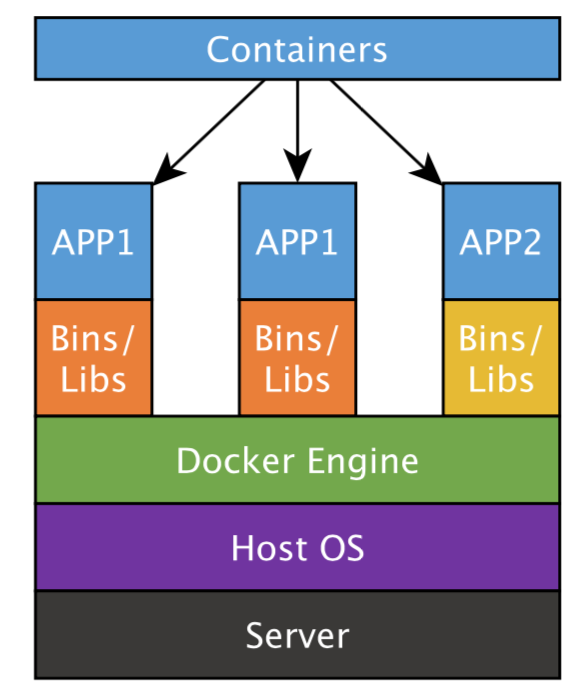
\includegraphics[width=0.45\textwidth]{Figures/containers.png}
    	\caption[Virtualización basada en contenedores]{Virtualización basada en contenedores: los contenedores comparten el sistema operativo del host y por lo tanto no necesitan una copia.}
    	\label{fig:contenedor-arch}
     \end{subfigure}
    ~ 
    \begin{subfigure}[b]{0.48\textwidth}
         \centering
    	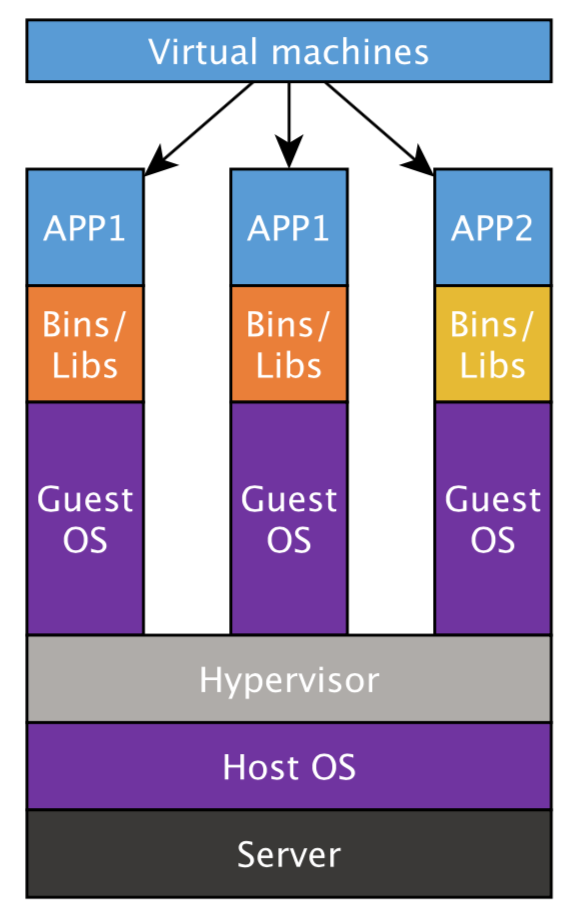
\includegraphics[width=0.45\textwidth]{Figures/virtual.png}
    	\caption[Virtualización basada en máquinas virtuales]{Virtualización basada en máquinas virtuales: las máquinas virtuales requieren un sistema operativo para cada uno.}
    	\label{fig:vm-arch}
     \end{subfigure}
        \caption[Comparación entre virtualizacion basada de contenedores y máquinas virtuales]{Dado que un contenedor comparte recursos, esto reduce significativamente el uso de almacenamiento en comparación a las máquinas virtuales.}
        \label{fig:virtualization}
\end{figure*}

Las diferencias entre la virtualización basada en contenedores y máquinas virtuales presentan características interesantes para la ejecución de aplicaciones y workflows. Dado que un contenedor comparte recursos con el sistema operativo, como las bibliotecas, esto reduce significativamente la necesidad de reproducir el código del sistema operativo, y significa que un servidor puede ejecutar varios ambientes con una sola instalación del sistema operativo. 
Por lo tanto, los contenedores son excepcionalmente ligeros: sólo tienen un tamaño de mega-bytes y sólo tardan unos segundos en arrancar. En comparación con los contenedores, las máquinas virtuales tardan minutos en funcionar y son un orden de magnitud mayor que un contenedor equivalente. \cite{padala2007performance,regola2010recommendations,felter2014updated}. A partir de esto nace la motivación de la utilización de contenedores con una alternativa para alcanzar la conservación física de los ambientes.
Docker es un proyecto open-source que utiliza la tecnología de los contenedores (libcontenedor) para ``construir, migrar y correr aplicaciones distribuidas". Actualmente utilizado por Yelp, Spotify, entre otros \cite{marmolnetworking}
Docker es una solución que simplifica el uso de los contenedores que han estado presente durante más de una década. Primero provee una interfaz simple y segura para crear y controlar contenedores \cite{bui2015analysis}, segundo permite a los desarrolladores empaquetar y correr sus aplicaciones de manera sencilla y además se integra con herramientas terceras que permiten administración y despliegue como Puppet\footnote{\url{https://puppet.com}}, Ansible \footnote{\url{https://ansible.com}} y Vagrant\footnote{\url{https://vagrant.com}}. Y diversas herramientas de orquestación como Mesos \footnote{\url{http://mesos.apache.org/}}, 
Shipyard \footnote{\url{https://shipyard-project.com/}},
Kubernetes \footnote{\url{https://kubernetes.io/}},
RancherOS \footnote{\url{http://rancher.com/rancher-os/}} y 
Docker Swarm \footnote{\url{https://docs.docker.com/swarm/}}.

Docker puede separarse en dos grandes componentes Docker Engine y Client.
Docker Engine es una herramienta liviana y portable para administrar la virtualización. Y Docker Client, provee una interfaz para interactuar con los contenedores con los usuarios a través de RESTful APIs\cite{bui2015analysis}.

\begin{figure}[t]
  \centering
  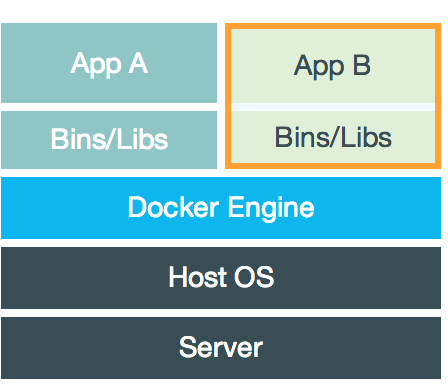
\includegraphics[width=0.3\textwidth]{Figures/docker.png}
    \caption{Arquitectura de Docker}
    \label{fig:docker}
\end{figure}

Docker utiliza una arquitectura de cliente-servidor, \emph{Docker Client} interactúa con \emph{Docker Daemon} y éste construye, maneja y corre los contenedores. Docker Client y Docker Daemon pueden correr en el mismo host o se puede conectar el cliente desde un host remoto. El cliente y el Daemon se comunican en forma de sockets o RESTful API \footnote{\url{https://docs.docker.com/introduction/understanding-docker/}}. 
Una imagen de Docker (\textit{Docker Image}) es una plantilla de solo lectura. Por ejemplo, una imagen puede contener las herramientas básicas de Ubuntu con Apache y una aplicación web instalada o simplemente el sistema operativo. Las imágenes son usadas para construir los contenedores. Y cuando el usuario crea cambios en el contenedor, este cambio no se realiza en la imagen, sino  que Docker añade una capa adicional con los cambios de la imagen\cite{bui2015analysis}. Por ejemplo, si el usuario utiliza una imagen base de Debian, luego añade el paquete emacs y luego añade el paquete apache, el estado de capas estaría representado por la figura \ref{fig:arquitectura}. Esto permite tener un proceso de distribución de imágenes más eficiente dado que solo es necesario distribuir las actualizaciones \cite{bui2015analysis}. El sistema de archivos descrito anteriormente se denomina una sistema de archivo basado en capas.

\begin{figure}[t]
  \centering
  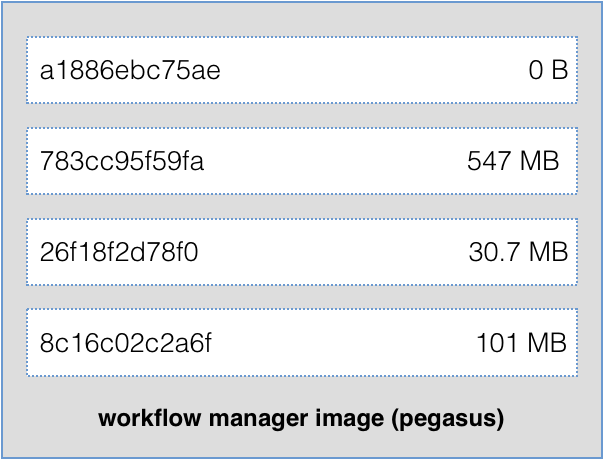
\includegraphics[width=0.4\textwidth]{Figures/docker-filesystems-multilayer}
    \caption[Capas de una imagen de Docker]{Las imágenes Docker con compuestas por capas. 
    La última capa (a1886ebc75ae) es la única capa en modo escritura.}
    \label{fig:arquitectura}
\end{figure}	


\subsection{Docker Hub}
Docker Hub es un repositorio que almacena dos tipos de repositorios oficiales y comunitarios. Los repositorios oficiales contienen imágenes públicas y verificadas de empresas y proveedores de software de renombre, como Canonical, Nginx, Red Hat y el propio Docker. Al mismo tiempo, los repositorios comunitarios pueden ser repositorios públicos o privados creados por usuarios y organizaciones individuales, que comparten sus aplicaciones y resultados. 

Usando ese repositorio y una línea de comandos, es posible descargar e implementar imágenes Docker localmente, ejecutando el contenedor en un entorno host, y ejecutando así el software dentro de la imagen. Los usuarios pueden crear y almacenar imágenes en el registro del Docker Hub, creando un archivo descriptor llamado Dockerfile o ampliando uno existente.  Este archivo describe cuáles son los comandos para construido la imagen y por lo tanto los paquetes de software que estarán dentro de la imagen, luego se construye la imagen y finalmente se sube al Docker Hub. Sin embargo, Docker Hub no controla qué paquetes hay en las imágenes, si la imagen se desplegará correctamente o si las imágenes pueden tener algún problema de seguridad. 
Así, las imágenes Docker funcionan como una caja negra, lo que significa que los usuarios saben sólo paquetes principales que se ejecutan dentro del contenedor pero no conocen los otros paquetes necesarios para ejecutarlo.
Hay dos maneras de subir imágenes a un repositorio de usuario, ya sea enviar la imagen desde un host local o automatizando ese proceso desde un repositorio Github \footnote{\url{https://github.com/}}. Para enviar una imagen al Docker Hub, los usuarios necesitan nombrar sus imágenes locales usando su nombre de usuario Docker Hub, y el nombre del repositorio que han creado. 
Después, los usuarios añaden múltiples versiones a un repositorio añadiéndole la versión \texttt{:<tag>}. 
Esta es toda la información que normalmente tienen las imágenes Docker en DockerHub, siendo por tanto casi imposible reproducir el entorno de ejecución si se modifica alguno de los paquetes de software utilizados dentro de las imágenes. 


DockerHub permite a las comunidades científicas almacenar y compartir, conservando el contenido de los contenedores, así como comprobar la identidad del editor y recuperar los contenedores de interés. Sin embargo, la información del contenido de cada repositorio no siempre es accesible de forma clara. 
Como la mayoría de las veces sólo se proporcionan descripciones cortas de los contenedores, no es fácil para el usuario entender qué componentes están instalados en ellos. 
Incluso cuando los archivos Dockerfile están disponibles, no son lo suficientemente intuitivos de entender cuáles paquetes están siendo desplegados por cada comando.

Además, es posible que en el contenedor existan algunos componentes que no estén especificados por el propio Dockerfile. Para abordar este problema proponemos un enfoque automático para analizar el contenido de un contenedor Docker y extraer la información sobre los componentes de software instalados en él. Esta información se convierte en datos semánticos, codificados como RDF bajo el conjunto de ontologías.

Los contenedores Docker consiste de un ambiente virtual: con archivos de usuarios y metadatos, cada contenedor es construido a partir de una imagen base como se mencionó anteriormente. 
Esta imagen indica la base del contenedor y se asocia un proceso inicial, él cual debe correr cuando el contenedor es iniciado.

La figura \ref{lst:simple-docker}describe los pasos incluidos en la creación de un contenedor.

\begin{figure*}
	\begin{lstlisting}[caption={Ejemplo de la ejecución de un contenedor utilizando la imagen Docker},label={lst:simple-docker},language=bash]
	docker run -i -t ubuntu /bin/bash
\end{lstlisting}
\end{figure*}

	\begin{itemize}
		\item \emph{Docker Client} le informa al Docker que debe correr un contenedor.
		\item En este caso el comando \texttt{/bin/bash} será el proceso \texttt{init} o 0 del contenedor
		\item Docker verifica la existencia de la imagen Ubuntu y sino existe en el host, entonces Docker descarga desde el repositorio ya sea privado o publico. Si la imagen existe entonces crea el contenedor.
		\item Asignar el sistema de archivos y montar la capa de escritura, para crear el contenedor debe realizarse en el sistema de archivos y añadir una capa en modo escritura en la imagen.
		\item Crea la interfaz de red que permite que contenedor pueda enviar y recibir paquetes con el host a través del puente (docker0).
		\item Asigna una dirección IP del conjunto de dirección IP disponibles al contenedor
		\item Dependiendo de la configuración de contenedor, Docker enviará a los registros de errores hacia el mismo servidor u otro externo.
	\end{itemize}

\subsection{Aislamiento y seguridad}
Para crear los ambientes virtuales Docker utiliza dos funcionalidades de Linux: \emph{namespaces}\footnote{\url{http://man7.org/linux/man-pages/man7/namespaces.7.html}} y \emph{cgroups}\footnote{\url{http://man7.org/linux/man-pages/man7/cgroups.7.html}}. \emph{cgroups} o \emph{control groups} proveen un mecanismo de contabilidad y limites de recursos que pueden utilizar los contenedores\cite{bui2015analysis}. Los \emph{namespaces} proveen del aislamiento para el contenedor. 
Cuando se crea un contenedor, Docker crea un conjunto de \emph{namespaces} para el contenedor. Los \emph{namespaces} utilizados por Docker son: mount (mnt) para el manejo del montaje, PID para el aislamiento de los procesos, net para el manejo de interfaces y IPC para acceder a recursos de IPC. 
Docker logra el aislamiento de los procesos separando los procesos en \emph{PID namespaces}.
\emph{PID namespaces} (añadido en el kernel \( \geq 2.6.3.2)\) logdando que un proceso que se encuentra en el contenedor solo pueda ver procesos que se encuentra en ese contenedor. Por lo tanto un atacante no puede observar procesos de otro contenedor, lo que aísla al contenedor este nivel \cite{bui2015analysis}.
Docker usa \emph{mount namespaces} o \emph{filesystem namespaces} para aislar los \emph{filesystems} asociados a los contenedores. De la misma forma que ocurre con los procesos, los eventos del sistema de archivos que ocurre en el contenedor sólo afectan a ese contenedor.

Cómo se menciono anteriormente, Docker utiliza \emph{cgroups} que permite especificar que \emph{device} puede ser utilizado con el contenedor. Esto bloquea la posibilidad de crear y usar \emph{device nodes} que puedan ser utilizados para atacar el host. Los \emph{device nodes} que son creados para cada contenedor por defecto: son: /dev/console, /dev/null, /dev/zero, /dev/full, /dev/tty*, /dev/urandom, /dev/random, /dev/fuse.
IPC (\emph{inter-process communication} es un conjunto de objetos para el intercambio de datos a través de los procesos, como semáforos, colas de mensajes, segmentos de memoria compartida. Los procesos corriendo en los contenedores utilizan \emph{IPC namespaces} que permite la creación de un \emph{IPC} separado y independiente para cada contenedor, con esto se previene que procesos en un contenedor interfieran con otros contenedores o el host.
Para cada contenedor, Docker crea una red independiente usando \emph{network namespaces}, compuesta de su propia IP, rutas, \emph{network devices}. Esto permite que el contenedor pueda interactuar con otro host a través de su propia interfaz.
Por omisión, la conexión se realiza gracias al host que provee un \emph{Virtual Ethernet bridge} en la máquina host, llamado docker0 que automáticamente realiza un \emph{forward} de los paquetes entre las interfaces. Cuando Docker crea un nuevo contenedor, se crea una interfaz de red virtual con un nombre único que se conecta con el \emph{bridge (docker0)} y con la interfaz \emph{eth0} del contenedor \cite{bui2015analysis}.
Además \emph{Cgroups} controla la cantidad de recursos como CPU, memoria, \emph{disk I/O} que el contenedor puede utilizar. 
Fijando estos parámetros se puede limitar los efectos de un dtaque de denegación de servicio (DDoS).

\section{Clair}\label{sec:clair}

Clair~\footnote{https://github.com/coreos/clair/} es un proyecto de código abierto para el análisis estático de vulnerabilidades en contenedores de aplicaciones (actualmente incluyendo appc \footnote{\url{https://coreos.com/rkt/docs/latest/app-container.html}} y Docker).
   
En intervalos regulares, Clair ingiere metadatos de vulnerabilidades un conjunto configurado de fuentes y los almacena en la base de datos. 
Para analizar las imágenes, los clientes utilizan la API de Clair y el sistema indexa sus imágenes; esto crea una lista de características presentes en la imagen y las almacena en la base de datos.

Clair define su propia terminología:

\begin{description}
	\item [Feature:] cualquier funcionalidad que éste presente en el sistema de archivos que sea una indicación de una vulnerabilidad (e.g. presencia de un archivo o paquete)
	\item [Feature Namespace:] contexto de \emph{feature} o vulnerabilidades (e.g. un sistema operativo o lenguaje)
	\item [Vulnerability Source (vulnsr):] el componente de Clair que rastrea los datos de vulnerabilidad y los importa a la base de datos de Clair
	\item [Vulnerability Metadata Source (vulnmdsrc):] el componente de Clair rastrea los metadatos de vulnerabilidad y los asocia con las vulnerabilidades en la base de datos de Clair
\end{description}

Clair se compone de distintos controladores (\emph{drivers}).

\begin{description}
	\item [featurefmt:] identifica el formato de las funcionalidades de una capa (e.g. apt).
	\item [featurens:] identifica cuáles son los \emph{namespaces} que son aplicables a la capa (e.g. ubuntu 16.04).
	\item [imagefmt:] determina la ubicación del sistema de archivos raíz de la capa (e.g. Docker).
	\item [versionfmt:] determina y compara los strings de la versión (e.g. rpm).
	\item [vulnmdsrc:] descarga los metadatos de las vulnerabilidades para ser procesados (e.g. National vulnerability database - NVD \footnote{\url{https://nvd.nist.gov/}} ) .
	\item [vulnsrc:] descarga las vulnerabilidades para un conjunto de \emph{namespaces} (e.g. \emph{Alpine Security Database of Backported fixes})
\end{description}

La figura \ref{table:clair-datasources} muestra los drivers implementados por Clair.

\begin{table}[t]
\begin{tabular}{|l|l|l|l|}
\hline
Fuente de datos             & Datos recolectados                                                                                                          & Formato & Licencia \\ \hline
Debian Security Bug Tracker & \emph{Namespaces:} Debian 6, 7, 8 y inestable                                                                               & dpkg    & Debian   \\ \hline
Ubuntu CVE Tracker          & \begin{tabular}[c]{@{}l@{}}\emph{Namespaces:} Ubuntu 12.04, 12.10,\\  13.04, 14.04, 14.10, 15.04, 15.10, 16.04\end{tabular} & dpkg    & GPLv2    \\ \hline
Red Hat Security Data       & \emph{Namespaces:} CentOS 5, 6, 7                                                                                           & rpm     & CVRF     \\ \hline
Oracle Linux Security Data  & \emph{Namespaces:} Oracle Linux 5, 6, 7                                                                                     & rpm     & CVRF     \\ \hline
Alpine SecDB                & \begin{tabular}[c]{@{}l@{}}\emph{Namespaces:} Alpine 3.3, Alpine 3.4, \\ \\ Alpine 3.5\end{tabular}                         & apk     & MIT      \\ \hline
NIST NVD                    & Metadatos genéricos de vulnerabilidades                                                                                     & N/A     & Pública   \\ \hline
\end{tabular}
\caption{Fuente de datos implementadas por Clair}
\label{table:clair-datasources}
\end{table}

\section{Sistemas de paquetes}

Un gestor de paquetes es un conjunto de herramientas de software qué automatiza el proceso de instalación, actualización, configuración y eliminación de programas para el sistema operativo de un ordenador de forma coherente.

Un gestor de paquetes se ocupa de paquetes, distribuciones de software y datos en ficheros de archivo. Los paquetes contienen metadatos, como el nombre del software, la descripción de su propósito, el número de versión, el proveedor, la suma de comprobación y una lista de dependencias necesarias para que el software funcione correctamente. 

Tras la instalación, los metadatos se almacenan en una base de datos de paquetes local. Esta base de datos se guarda en un archivo en el sistema de archivos. Por lo tanto, la información de los componentes del software de una imagen se encuentra en cada una de sus capas.
Dependiendo del sistema de paquetes, se puede utilizar otras herramientas para obtener mayor información utilizando la información que se encuentra en la base de datos.

A continuación se describe los sistemas de paquetes populares

\subsection{rpm}\label{sub:rpm}
\emph{RPM Package Manager} (RPM) es un sistema de empaquetado abierto, que se ejecuta en Red Hat Enterprise Linux así como en otros sistemas Linux y UNIX.
El archivo de base de datos de rpm se encuentra ubicado en \verb|/var/lib/rpm/Packages|. La información disponible en ese archivo es: Nombre, Versión, Lanzamiento, Arquitectura, Fecha de instalación, Grupo, Tamaño, Licencia, Firma, RPM de origen, Fecha de construcción,  Host de reconstrucción, Proveedor del paquete, URL, Resumen y  Descripción.
\subsection{dpkg}\label{sub:dpkg}

Debian Package Manager (dpkg) es un sistema de gestión de paquetes en el sistema operativo libre Debian y sus numerosos derivados. dpkg se utiliza para instalar, eliminar y proporcionar información sobre los paquetes .deb. 

El archivo de base de datos de dpkg se encuentra ubicado en \verb|/var/lib/dpkg/status| utilizando formato texto plano.  La información disponible es: Paquete, Estado, Prioridad, Sección, Tamaño de la instalación, Encargado del mantenimiento, Arquitectura, Fuente, Versión, Reemplaza a otro paquete, Dependencias y Recomendaciones.

\subsection{apk}\label{sub:apk}

apk es un sistema de gestión de paquetes en el sistema operativo Alpine. Alpine se ha convertido una distribución de Linux muy utilizada en contenedores debido a que la imagen tiene un tamaño menor a los 10 MB.
El archivo de base de datos de apk se encuentra ubicado en \verb|/lib/installed|. La información disponible se basa la especificación de apk \footnote{\url{https://wiki.alpinelinux.org/wiki/Apk_spec}}: Arquitectura, Suma del pull, Dependencias, Ruta de archivos, Tamaño, Licencia, Nombre del paquete, Descripción, URL, git commit del paquetes, tiempo de construcción, entre otros. 

\subsection{Conda}\label{sub:conda}
Conda es un gestor de paquetes, dependencias y entornos para lenguajes Python, R, Ruby, Lua, Scala, Java, JavaScript, C/ C++, FORTRAN y que es ampliamente utilizado en entornos de \textit{Jupyter notebook}.

El archivo de base de datos de Conda se encuentra ubicado en \verb|conda/history| según la posición del ambiente. La información disponible se basa la especificación de Conda \footnote{\url{https://conda.io/docs/user-guide/tasks/build-packages/package-spec.html}}: Nombre, versión, versión de construcción, número de construcción, dependencias, arquitectura, plataforma y archivos.

\section{Web Semántica}

La web semántica es un extensión \emph{World Wide Web} añadiendo un conjunto de estándares diseñado por la \emph{World Wide Web Consortium} con el objetivo de la creación de tecnologías para publicar datos legibles por aplicaciones informáticas. 
Para lo lograr lo anterior, se añaden metadatos semánticos y ontologías para describir el contenido y generar relaciones entre los datos, esta representación se realiza de una manera formal.
Consecuentemente, la información disponible pueden ser procesadas de manera automática mejorando la inter operatividad entre distintos sistemas informáticos que realizan búsquedas sin operadores humanos.
El término fue acuñado por Tim Berners-Lee y describe una red de datos que puede ser procesada por máquinas. Además, en \cite{berners1992world} se afirma la necesidad de que los datos se transformen desde objetos legible por personas a información semántica diseñada para las máquinas.
Es por ello que la web semántica ha definido diversos estándares para construir una descripción formal de los conceptos, términos y relaciones. Estos estándares definidos por W3C incluyen: RDF, RDFS, SPARQL, Notation3 (N3), N-Triples, Turtle y OWL.

\subsection{RDF}\label{sw:rdf}
RDF (del inglés \emph{Resource Description Framework}) es un modelo estándar para el intercambio de datos en la Web. 
Distintas especificaciones se han publicado: en 1999 se adopto como una recomendación del W3C y las especificaciones 1.0 y 1.1 se publicaron en 2004 y 2014 respectivamente \cite{bikakis2013semantic}.

RDF extiende la estructura de enlace de la Web para usar URIs para nombrar la relación entre cosas. Un triple tiene la forma de expresión  $\langle sujeto, predicado, objeto \rangle$. Donde el $sujeto$ indica el recurso, el $predicado$ nombra la relación entre el $sujeto$ y $el objeto$

\subsection{RDFS}
RDFS (de las siglas del inglés \emph{Resource Description Framework Schema},
también llamado RDF Schema) es un vocabulario que extiende RDF utilizando un
conjunto de clases y propiedades que mejoran la creación de modelos como son:
\tt{Class} para declarar clases, \tt{subClassOf} para denotar herencia,
\tt{range} y \tt{domain} para el rango y dominio de cierta propiedad
(\tt{rdf:Property}), entre otras.

En 1998 se presento y fue introducido como recomendación del W3C en 2004
\cite{bikakis2013semantic}.

\subsection{OWL}

OWL (del inglés \emph{Web Ontology Language}) es un lenguaje semántico para publicar y compartir ontologías complejas en la W3C, OWL se desarrolla como una extensión de vocabulario de RDF (Resource Description Framework). 
Se han publicados versiones de OWL. La primera OWL publicada el 2004 y la segunda version ``OWL 2'' fue publicada el 2009 como una revisión y extensión de la versión inicial Usualmente cuando se habla de ``OWL'' se refiere a la versión a la versión del 2004.


En el siguiente capítulo se exponen los problemas abiertos de investigación y los objetivos e hipótesis del presente trabajo.

\chapter{Objetivos de trabajo}\label{sec:objetivos} 
El principal objetivo de este trabajo es complementar enfoques existentes para la reproducibilidad científica en el área de las ciencias de la computación. Para ello, se propone un nuevo enfoque para conservar el ambiente de ejecución del experimento científico.
Se ha identificado los problemas abiertos, en orden de definir los objetivos de trabajo. Luego, estos objetivos se ven formalizados por un conjunto de hipótesis. Y además, se define un conjunto de hechos que se asumen para restringir el campo de aplicación de la propuesta.

%--------------------------------------------
%	SECTION OPEN RESEARCH PROBLEMS
%-------------------------------------------

\section{Problemas de investigación abierto}
\begin{itemize}
	\item Problema 1: La infraestructura computacional utilizada por un workflow científico se encuentra predefinida. Por lo tanto, no existe una definición de los recursos de la infraestructura para ejecutar el experimento. Consecuentemente, pueden existir dificultades para lograr la reproducción del experimento. 
	\item Problema 2: La conservación física de los ambientes computaciones permite mantener y compartir fácilmente el ambiente con la comunidad. Sin embargo, se ha descartado debido a tres problemas: 
		1. Alta utilización de almacenamiento por parte de las máquinas virtuales, 
		2. El acceso a los datos almacenados está sujetos a políticas de la organización 
		y 3. Existe un proceso de decaimiento en tiempo.
		Sin embargo, no se ha estudiado el uso de containers para solucionar el problema.
	\item Problema 3: Los enfoques actuales anotan los pasos de construcción de los ambientes computacionales de forma indirecta, por lo tanto, recaen en el científico 
\end{itemize}

%--------------------------------------------
%	SECTION HIPÓTESIS
%-------------------------------------------
\section{Hipótesis}

En función a los problemas abiertos detectados, se definen las siguientes hipótesis:

\begin{itemize}
	\item Un proceso automático puede describir los requerimientos de ambiente computacional y codificarlo en un formato compartible utilizando modelos semánticos.
	\item La descripción de contenedores utilizando modelos semánticos permite la reproducción del ambiente de un experimento científico.
\end{itemize}
%--------------------------------------------
%	SECTION OBJETIVOS
%-------------------------------------------


\section{Objetivos}

Para enfrentar los problemas abiertos se definen los siguientes objetivos. Estos objetivos permiten la verificación de la hipótesis y ser una guía para el desarrollo.

\begin{itemize}
	\item Lograr conservación física y lógica de los ambientes computaciones de un experimento usando Containers
	\item Implementar un proceso automático capaz de leer la descripción del ambiente y especificar uno nuevo.
	\item Integrar un sistema que permita el despliegue de estos ambientes computacionales en proveedores de infraestructura e instalar el software apropiado basado al plan de despliegue.
\end{itemize}

\subsection{Objetivos específicos}

\begin{itemize}
	\item Adaptar y mejorar modelos estándares que describen ambientes computacionales científicos para incluir virtualización basada en contenedores.
	\item Designar una framework para anotar los componentes de ambiente del experimento usando modelos semánticos.
\end{itemize}

\section{Suposiciones}

\begin{itemize}
	\item Las técnicas de virtualización basadas en contenedores son una tecnología estable. Por lo tanto, las herramientas utilizadas estarán disponibles a largo plazo. Al igual que los sitios de almacenamiento de repositorios o soluciones de software que soportan la gestión de recursos virtualizados.
	\item Los componentes de software anotados será los cuáles sean instalados por sistemas de paquetes. Los componentes de software que sean binarios serán solamente anotados en los pasos de construcción. 
\end{itemize}
\chapter{Conservación del ambiente de ejecución}

En este trabajo, se argumenta que las descripciones de los ambientes computacionales son necesarias para la reproducción del experimento. Además, la información debe ser la suficiente para comparar y detectar las diferencias entre el ambiente original y el reproducido.

Dado que las imágenes Docker son ambientes aislados e independientes, asumimos que los componentes de software dentro del contenedor si están relacionados al experimento y no existen componentes relacionados a otros experimentos dentro del mismo contenedor.
Por esta razón, se asegura que las anotaciones no presentarán ruido de otras herramientas o dependencias asociadas, causadas por entremezclar la ejecución de otros experimentos con otros requisitos computacionales en el mismo contenedor.
Para realizar una anotación automática de los paquetes instalados, se propone e implementa un sistema de anotación automático. El sistema requiere el nombre de una imagen existente en un repositorio de DockerHub y los datos del repositorio Git que almacena el archivo Dockerfile. 

Los pasos asociados del sistema anotación:
\begin{enumerate}
	\item Consultar al repositorio de imágenes Docker los metadatos de la imagen. 
	\item Anotar los metadatos utilizando la ontología propuesta.
	\item Descargar cada una de las capas asociadas a la imagen Docker.
	\item El sistema anotador consulta a Clair, Clair monta cada una de capas de la imagen, detecta los componentes de software instalados a través el sistema de paquete.
	\item Obtener la información desde Clair y anotar los datos obtenidos por Clair según la ontología.
	\item Guardar los datos en una base de datos RDF.
\end{enumerate} 

%----------------------------------
% 4.1 Semantic models
%----------------------------------
\section{Modelos semánticos}\label{s4.1}
     
En \cite{santana2017reproducibility}, los autores proponen \emph{The Workflow Infrastructure Conservation Using Semantics ontology (WICUS)}. WICUS es ontología OWL2 (Web Ontology Language) que implementa la conceptualización de los principales dominios de la infraestructura computacional. Estos son: Hardware, Software, Workflow y recursos de computo.
Los autores definen que los workflows científicos requieren un conjunto de componentes de software, y los investigadores deben conocer cómo desplegar estos componentes para lograr ambiente equivalente.\todo[inline]{describe un p[oco mejor tu contribución con la ontología, tiene que quedar claro que esto también es una contribución, sobre todo el detalle más fino que logras}
Considerando que la ontología está relacionada con nuestro trabajo, se utiliza algunas clases y relaciones desde la ontología WICUS descriptas a continuación:

\begin{description}
	\item [DeploymentPlan:]  Un plan de despliegue está compuesto de todos los pasos. Y el plan de despliegue le permite entender al investigador cuáles fueron los pasos requeridos para construir el ambiente computacional.
	\item [DeploymentStep:] Cada paso de despliegue es representado por una línea de comando que realiza la instalación, descarga o configuración del ambiente. La información se obtiene desde el archivo DockerFile
	\item [SoftwareComponent:] Es un componente de software instalado sin una versión específica. 
\end{description} 

La ontología propuesta define el recurso \texttt{dockerpedia:SoftwarePackage} como una subclase de \texttt{wicus:SoftwareComponent} para definir los componentes instalados por el gestor de paquetes del sistema operativo u otro.
Cada \texttt{wicus:SoftwareComponent} tiene una relación \texttt{dockerpedia:hasVersion} o \texttt{dockerpedia:isVersionOf} que muestra la versión del software instalado.
El recurso \texttt{dockerpedia:PackageVersion} puede estar afectado por vulnerabilidades representadas por el recurso \texttt{dockerpedia:SoftwareVulnerability}. Y las versiones que reparan la vulnerabilidad se encuentran representadas por \texttt{dockerPedia:SecurityRevision}.
Una imagen Docker se representa por \texttt{dockerpedia:SoftwareImage} y sus capas por el recurso \texttt{dockerpedia:ImageLayer}. Los paquetes instalados en la imagen están relacionado por \texttt{vocab:ContainsSoftware} con su imagen.
Finalmente, el sistema operativo es representado por el recurso \texttt{dockerpedia:OperatingSystem} y cada imagen y capa de la imagen está asociado al recurso.
\todo[inline]{que logras con estas clases?}

Una versión completa de la ontología se encuentra disponible en nuestros repositorios \footnote{\url{https://github.com/dockerpedia/ontology/}} y la versión resumida se observa en la figura ~\ref{fig:ontology}. 

\begin{figure}[t]
  \centering
    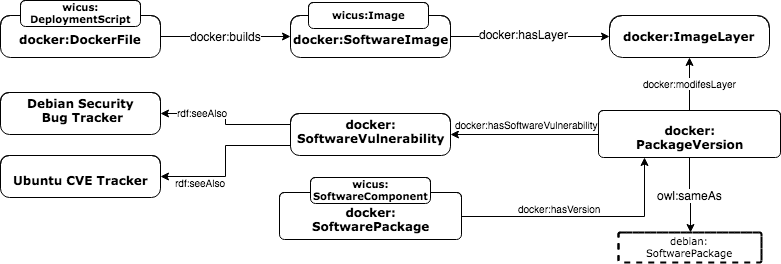
\includegraphics[width=1\textwidth]{Figures/dockerOntologyBasic.png}
      \caption{Ontología resumida para DockerPedia.}
     \label{fig:ontology}

\end{figure}

%----------------------
% 4.2 Annotator
%-----------------------
\section{Anotador}\label{s4.2}

El servicio de anotación propuesto cuenta con una interfaz REST para recibir el nombre y la versión de la imagen Docker relacionada con el experimento científico. 
Para almacenar e interactuar con los datos el sistema de anotación utiliza a Apache Jena~\footnote{\url{https://jena.apache.org/}}. Apache Jena es un framework Java gratuito\todo[inline]{las cosas no son gratis, son libres! verificar la licencia} y de código abierto para la construcción de aplicaciones de Web Semántica y Datos Enlazados. El sistema anotador construye los triples relacionados con el experimento, imagen, capas, componentes de software y vulnerabilidades y se envían usando la API de Apache Jena que serializa los triples utilizando formatos populares como RDF/XML o Turtle.
Es importante remarca que la arquitectura permita la utilización de otras herramienta en caso que Apache Jena no cumpla con los requerimientos de escalabilidad.

El sistema anotación realiza dos tipos de anotaciones: Componentes de software y pasos de construcción.


%--------------------------------------------
% 4.2.1 Building steps annotations
%---------------------------------------------
\subsection{Anotaciones de los pasos de construcción}\label{s4.2.1}

Anotamos el plan de despliegue (Deployment Plan) usando dos métodos. El primer método obtiene los pasos desde el archivo Dockerfile entregado por el usuario, esto permite obtener los pasos y la ubicación de archivo en el repositorio. 
Usando este método se asegura la reconstrucción del ambiente debido a que cualquier archivo necesario por Dockerfile se encuentra en el repositorio Git.
Sin embargo, un usuario puede construir una imagen sin compartir el archivo Dockerfile. En ~\cite{DBLP:conf/semweb/OsorioAV18a} se reporta que sólo el 30\% de las imágenes Docker en DockerHub vincula su archivo Dockerfile. 
Por lo tanto, si no existe información del Dockerfile el sistema anotación utiliza el manifiesto de la imagen Docker. Sin embargo, si el usuario no comparte su repositorio con los archivos no podemos asegurar la reproducibilidad por la falta del código o configuración y la información se guarda para referencia del investigar.
Respecto al manifiesto,  según \footnote{\url{https://docs.docker.com/registry/spec/manifest-v2-2/}} el manifiesto de la imagen provee la configuración y el conjunto de las capas y pasos de construcción de la imagen.
 
 
Algunos atributos relevantes del manifesto son:

\begin{description}
	\item [name:] \textit{string} nombre de la imagen
	\item [tag:] \textit{tag} versión de la imagen
	\item [architecture:] \textit{string} arquitectura del servidor en cuál la imagen ha sido construido. Esta información actualmente no es utilizada por Docker.
	\item [fsLayers:] \textit{array} lista de las capas que componente la imagen.
		La estructura contiene los siguiente campos:
		\begin{description}
			\item [blobSum:] es un identificador utilizando una función de hash sha256 para cada capa de la imagen 
		\end{description}
	\item [history]: \textit{array} Es una lista de datos históricos no estructurados para la compatibilidad con la v1. Contiene ID de la capa de imagen y el ID de las capas principales de la capa. El historial es una estructura que consta de los siguientes campos:
	\begin{description}
		\item[v1Compatibility]:  \textit{string} V1Compatibilidad es la información de compatibilidad de V1 en bruto. Esto contiene el objeto JSON que describe la V1 de esta imagen. Una V1Compatibilidad es una estructura que consta de los siguientes campos:
		
		\begin{description}
			\item [Id:] \textit{string} ID de la capa utilizando hash sha256			\item [Parent:] \textit{string} ID de la capa madre utilizando hash sha256
				\item [ContainerConfig:] \textit{string} El comando que construyó la capa
		\end{description}
	\end{description}
\end{description}



%--------------------------------------------
% 4.2.2 Software Components annotations
%---------------------------------------------
\subsection{Anotaciones de componentes de software}\label{s4.2.2}

La descripción de los componentes de software es fundamental para realizar cuantificar la similitud entre dos o más ambientes computacionales.
Un enfoque común para detectar los componentes de software guardar o detectar los comandos que realizan la instalación de software. Por ejemplo, la figura \ref{lst:tensorflow} muestra los comandos para instalar los componentes de la imagen TensorFlow. 
\begin{figure*}
	\begin{lstlisting}[caption={Ejemplo de instalación de dependencias para la imagen TensorFlow},label={lst:tensorflow},language=bash]
apt-get install -y --no-install-recommends \
        build-essential \
        curl \
        libfreetype6-dev \
        libhdf5-serial-dev \
        libpng12-dev \
        libzmq3-dev \
        pkg-config \
        python \
        python-dev \
        rsync \
        software-properties-common \
        unzip	
\end{lstlisting}

\end{figure*}


El enfoque detectaría los componentes: \verb|build-essential|, \verb|curl|, \verb|libfreetype6-dev|, \verb|libhdf5-serial-dev|, \verb|libpng12-dev|, \verb|libzmq3-dev|, \verb|pkg-config|, \verb|python|, \verb|python-dev|, \verb|rsync|, \verb|software-properties-common| y  \verb|unzip|. Sin embargo, este enfoque no obtiene información sobre las versiones o las dependencias del software. Utilizando el  enfoque propuesto, se puede terminar que el línea anterior instala 184 paquetes.



Otro enfoque  para lograr la anotación de los componentes de software es utilizar los gestores de paquetes del sistema. Los gestores que paquetes se clasifican en dos tipos: gestor de paquetes del tipo sistema y general:

\begin{description}
	\item  [Gestor de paquetes de sistema:] son aquellos vinculados al sistema operativo (e.g., apt de familia Debian, yum de familia RedHat).
	\item [Gestor de paquetes generales:] son aquellos externos que normalmente son utilizados para instalar componentes de software de terceros ó un lenguaje especifico (e.g., python, conda, npm). Por ejemplo, conda es un sistema paquete frecuentemente utilizado por investigadores al estar relacionado con Jupyter Notebook.
\end{description}


Es por ello que se utiliza Clair que fue introducido en la sección  \ref{sec:clair}, éste permite la detección componentes de software y vulnerabilidades dentro de una imagen de un contendor.
En este trabajo se utiliza Clair para detectar los componentes de software debido a que (i) no se necesita ejecutar el contenedor para detectar los componentes de software, (ii) no necesita instalar componentes de software extras dentro de la imagen y por lo tanto no se añade ruido al sistema, (iii) permite la extensión a otro tipo de sistema de contenedores como Singularity\footnote{\url{https://www.sylabs.io/docs/}}~\cite{kurtzer2017singularity} y (iv) el análisis es realizado por capas, lo que permite re usar análisis de otras capas ya analizadas.

Además, como prueba de generalidad se extiende Clair para detectar los paquetes instalados por Conda en la imagen.  
Sin embargo, Clair no cumple totalmente las necesidades para solucionar los problemas de anotación dado que Clair no considera múltiples detectores en la misma imagen y los componentes de software detectados son generados a partir de diferencias.
Por ejemplo, si se supone una imagen que está compuesta de dos capas: A y B donde A es padre de B y Clair presenta dos detectores \texttt{Alpha} y \texttt{Beta}. Donde el detector \texttt{Alpha} detecta componentes de software en el archivo \verb|/etc/a| y  \texttt{Beta} detecta componentes de software en el archivo \verb|/etc/b|. Si en la capa A, \texttt{Alpha} lista el software \verb|1| en \verb|/etc/a| y \texttt{Beta} lista \verb|2| en  \verb|/etc/b|. Y luego, en la capa B, \texttt{Beta}  lista \verb|2| y \verb|3| en  \verb|/etc/b|. El resultado de las diferencias será: 

\begin{enumerate}
	\item A añadió a \verb|1| y \verb|2|. Dado que observa el componentes de software en \verb|/etc/a| y \verb|/etc/b|
	\item  B añadió a \verb|3| y se mantuvo \verb|2| dado que observan en \verb|/etc/b|. Y se removió \verb|1| porque no hay archivo \verb|/etc/a|
\end{enumerate}

Pero si \verb|/etc/a| no tuvo cambios, el archivo no se ve incluye en la capa hija. Y no significa que el \verb|1| fuese removido. 
La casual del problema es que Clair añade y remueve paquetes sin considerar los detectores que detectaron los componentes de software. 
Consecuentemente, en esta propuesta se utiliza una copia del proyecto Clair que discrimina según el sistema de paquete que instaló el componente para permitir múltiples sistemas de paquetes de la imagen. El proyecto se encuentra disponible en el repositorio de DockerPedia \footnote{\url{https://github.com/dockerpedia/clair}}.

En la figura  \ref{fig:packages-pegasus} se muestra triples de algunos de los paquetes instalado en la imagen de un workflow construido con Pegasus, en la figura \ref{fig:vulnerability-pegasus} se muestra sus vulnerabilidades.
\begin{figure}[t]
    \hspace*{-4cm}   
    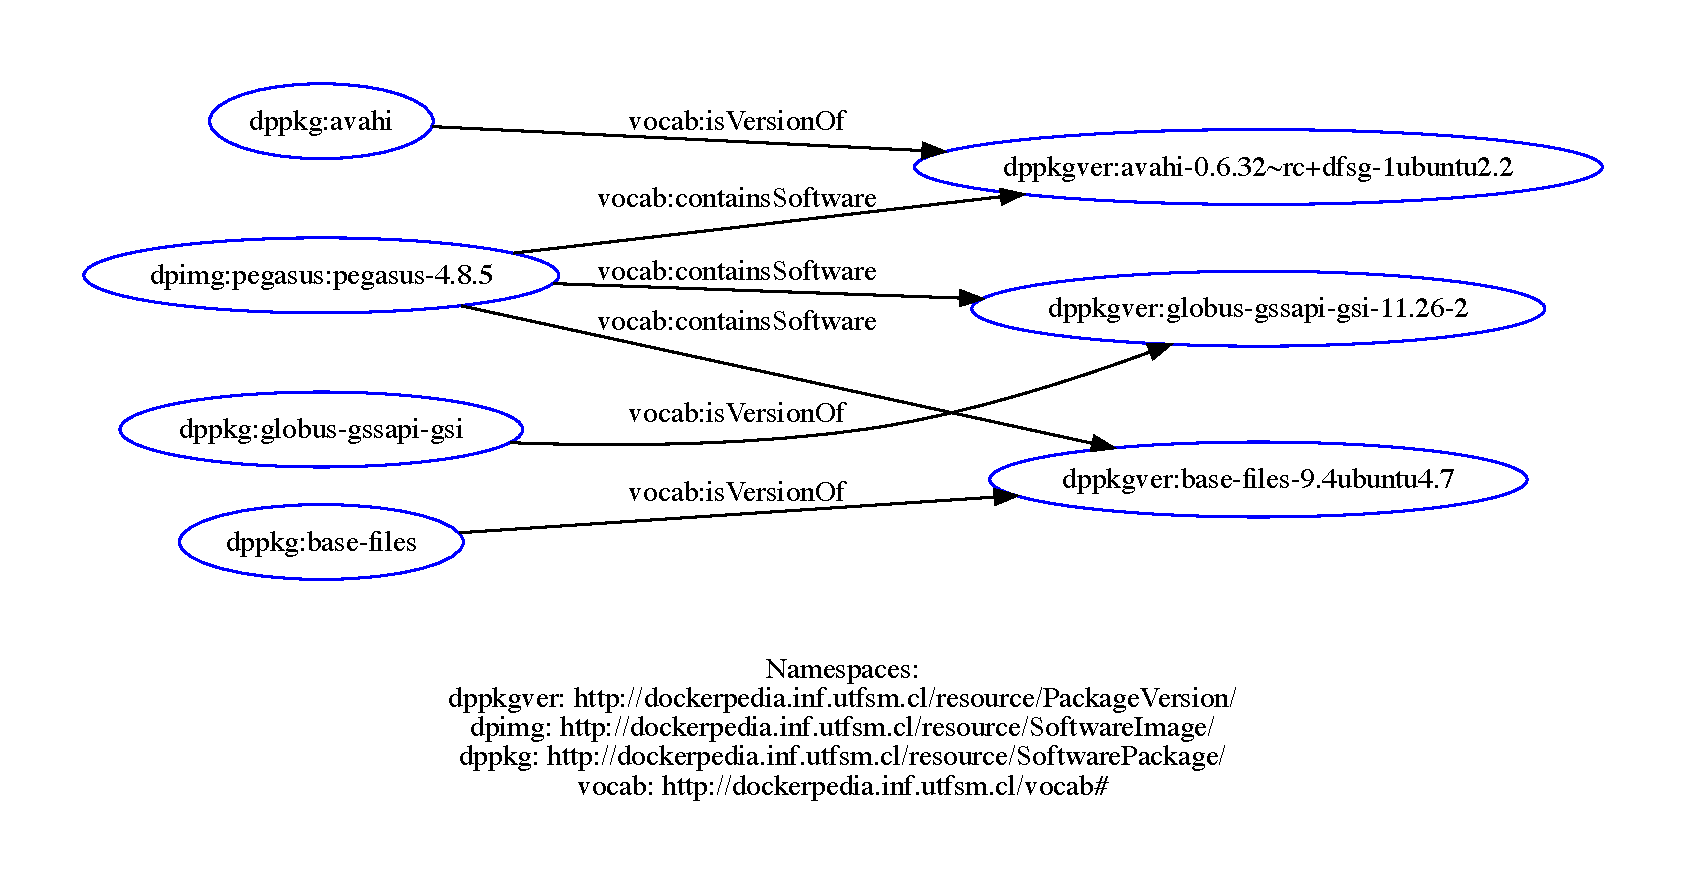
\includegraphics[width=1.3\textwidth]{Figures/packages}
     \caption[Paquetes de la imagen Pegasus]{Ejemplo de triples que muestran los componentes de software de la imagen Pegasus}
    \label{fig:packages-pegasus}
      
\end{figure}

\begin{figure}[t]
    \hspace*{-4cm}   
    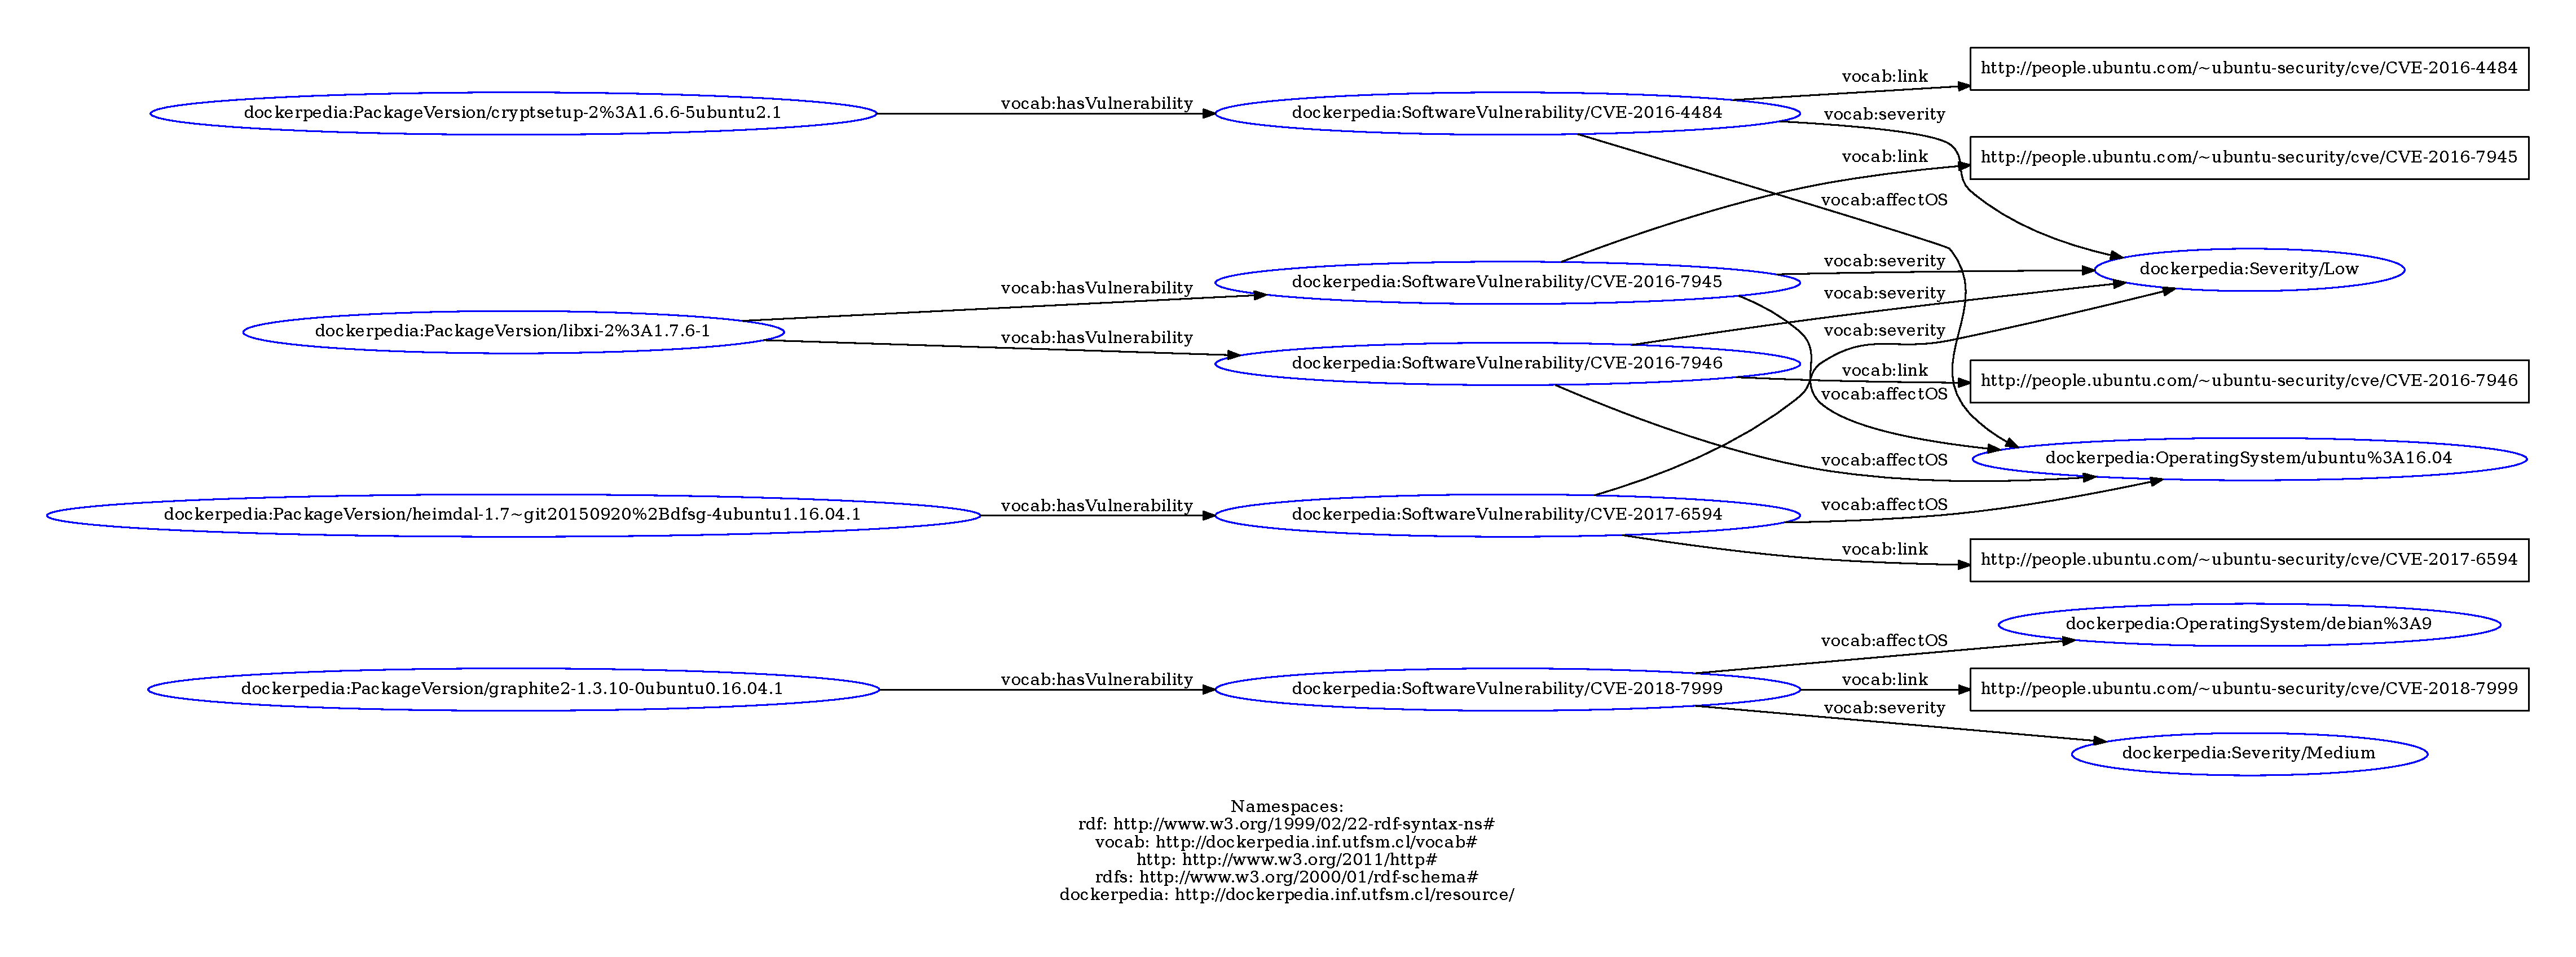
\includegraphics[width=1.3\textwidth]{Figures/packages-vuln}
      \caption[Paquetes y vulnerabilidades de la imagen Pegasus]{Vulnerabilidades y paquetes vulnerables de la imagen Pegasus}
    \label{fig:vulnerability-pegasus}
\end{figure}

\todo[inline]{termina los capítulos con un resumen de lo que has hecho, e introduciendo el siguiente, para que el lector siga con la curiosidad de qué viene después. Tienes que pensar también que el lector primero irá a la introducción del capítulo, después a las conclusiones de ese mismo capítulo y luego mirará el contenido si le interesa, tal y como pasa con el documento en general y como dice el libro Trees Maps and Theorems}
\chapter{Experimentación y evaluación}
%-----------------------------------------------
% 5.1 Scientific workflows
%-----------------------------------------------
%\todo[inline]{necesitas una introducción al capítulo, lo que vas a contar. Es lo mismo que pone en Trees Maps and theorems. Además, deberías empezar diciendo: esto es lo que hace un científico cuando construye y ejecuta un workflow de datos. No se entiende mucho esta sección.}


En este capítulo se introduce la experimentación para evaluar las hipótesis introducidas en el capítulo
\ref{sec:objetivos}. 
Para ello se diseña y se ejecuta un proceso de experimentación sobre un conjunto de workflows reales.
El proceso busca reproducir ambientes computacionales reales mediante el enfoque de conservación y el proceso de anotación propuesto. 
En otras palabras, se busca evaluar la propuesta considerando que los workflows experimentales necesitan garantizar que exista suficiente información sobre los experimentos para permitir la reconstrucción por un tercero, replicando sus resultados sin ninguna información adicional del autor original ~\cite{garijo2013quantifying}.
Por esta razón, se seleccionó un conjunto de experimentos computacionales representados por workflows. El conjunto incluye cinco workflows de distintos dominios de la ciencia que utilizan tres sistemas de manejo de workflows científicos (WMSs) distintos.
Luego, se anota el ambiente de computacional de cada workflow y es reproducido utilizando diferentes proveedores de Cloud y un ambiente local.

\section{Construcción de imágenes}\label{s5.1}

Para validar la propuesta y su aplicación en el contexto de workflows científicos, se ha seleccionado un subconjunto de workflows y sistemas de manejo de workflows científicos (WMS) 
El subconjunto ha sido seleccionado bajo los criterios de: nivel de utilización de WMS, la diversidad de lenguajes utilizados en el conjunto, y disponibilidad de los materiales del workflow. 

Los materiales de workflow son: los datos, el código y la documentación. La documentación permite el estudio de los componentes de software necesarios para la ejecución del ambiente. Y los datos y el código permiten la ejecución y obtención de los resultados.
Además para entender los requisitos del workflow, se inspecciona la las anotaciones manuales generadas por WICUS \cite{santana2017reproducibility} para los workflows comúnes.

Para cada WMS, se construye una imagen estándar. En consecuencia, un investigador puede importar esta imagen e instalar los componentes de software relacionados con el workflow.
Esto se puede conseguir utilizando la instrucción \texttt{FROM} de Dockerfile. Por ejemplo, si un experimento utiliza Pegasus como WMS, la imagen de experimento importará la imagen Pegasus.
Esto permite no almacenar una copia de las capas de Pegasus por cada workflow y disminuir el uso de disco.
En caso que el WMSs no distribuya su software utilizando Docker, se construye la imagen: esto incluye encontrar los componentes de software, las versiones necesarias de ellos, y las configuraciones requeridas. Lo mismo se realiza para cada workflow. 
Finalmente, se construye un repositorio Git en GitHub \footnote{\url{https://github.com/}} para cada WMSs y workflows con los archivos requeridos: DockerFile, configuraciones y otros.

Además, cada Dockerfile incluye información sobre la imagen utilizando el estándar de la Open Container Initiative \footnote{\url{https://www.opencontainers.org/}} Esta información es:

\begin{description}
   \item[org.opencontainers.image.created:] fecha y hora en la que se construyó la imagen (string, fecha y hora según la definición de RFC 3339).
    \item [org.opencontainers.image.authors] datos de contacto de las personas u organizaciones responsables de la imagen (lista de forma libre)).
    \item [org.opencontainers.image.url] URL para encontrar más información sobre la imagen (string).
    \item [org.opencontainers.image.documentation] URL para obtener documentación sobre la imagen (string).
    \item [org.opencontainers.image.source] URL para obtener el código fuente para construir la imagen (string).
    \item [org.opencontainers.image.version] versión del software empaquetado
        La versión puede coincidir con una etiqueta o tag en el repositorio de código fuente versión podría ser compatible con el versionado semántico.
    \item [org.opencontainers.image.revision] Identificador de revisión de control de origen para el software empaquetado.
    \item [org.opencontainers.image.vendor] Nombre de la entidad distribuidora, de la organización del artículo o del individuo.
    \item [org.opencontainers.image.licenses] Licencia(s) bajo la(s) cual(es) el software contenido se distribuye.
    \item [org.opencontainers.image.ref.name] Nombre de la referencia de un objetivo (string).  
    \item [org.opencontainers.image.title] Título de la imagen legible por el ser humano (string)
    \item [org.opencontainers.image.description] Descripción legible por un ser humano del software empaquetado en la imagen (string)
\end{description}


\section{Experimentos computacionales}\label{s5.1}


Para la experimentación se ha seleccionado un conjunto de experimentos de computaciones, éste se compone de cinco experimentos provenientes de áreas de astronomía, biología, sismología y geología.
Y se utilizaron tres WMSs: Pegasus~\cite{DBLP:journals/fgcs/DeelmanVJRCMMCS15}, dispel4py~\cite{DBLP:conf/eScience/FilgueiraKAKSS15} y WINGS~\cite{DBLP:journals/expert/GilRKGGMD11}. 
Al continuación se introducen los experimentaciones computaciones con su respectivo workflow.


\subsection{Pegasus}

Pegasus~\cite{DBLP:journals/fgcs/DeelmanVJRCMMCS15} es un WMS capaz de gestionar flujos de trabajo compuestos por millones de tareas, registrando datos sobre la ejecución y resultados intermedios. 
Pegasus lee las descripciones del flujo de trabajo de los archivos DAX. El término DAX es la abreviatura de ``Directed Acyclic Graph in XML". DAX es un formato de archivo XML que tiene sintaxis para expresar trabajos, argumentos, archivos y dependencias. Para crear un DAX es necesario escribir código para un generador de DAX.\\
Pegasus opcionalmente utiliza HTCondor como administrador de tareas. Por lo tanto, se construye dos versiones para la imagen de Pegasus; una versión tiene instalado el paquete condor y otra sin él. La justificación de decisión recae en permitir a los científicos utilizar una imagen simple si es necesario.
El paquete Pegasus ha sido obtenido del repositorio oficial~\footnote{\url{http://download.pegasus.isi.edu/wms/download/debian}}.
Y  al estudiar la documentación, se detectó los siguientes requisitos: Java (la versión Java depende de la versión pegasus), Python y Perl. La figura \ref{fig:pegasus-deps} muestra las dependencias especificadas tanto por el sistema de paquetes y documentación.

\begin{figure}[t]
\centering
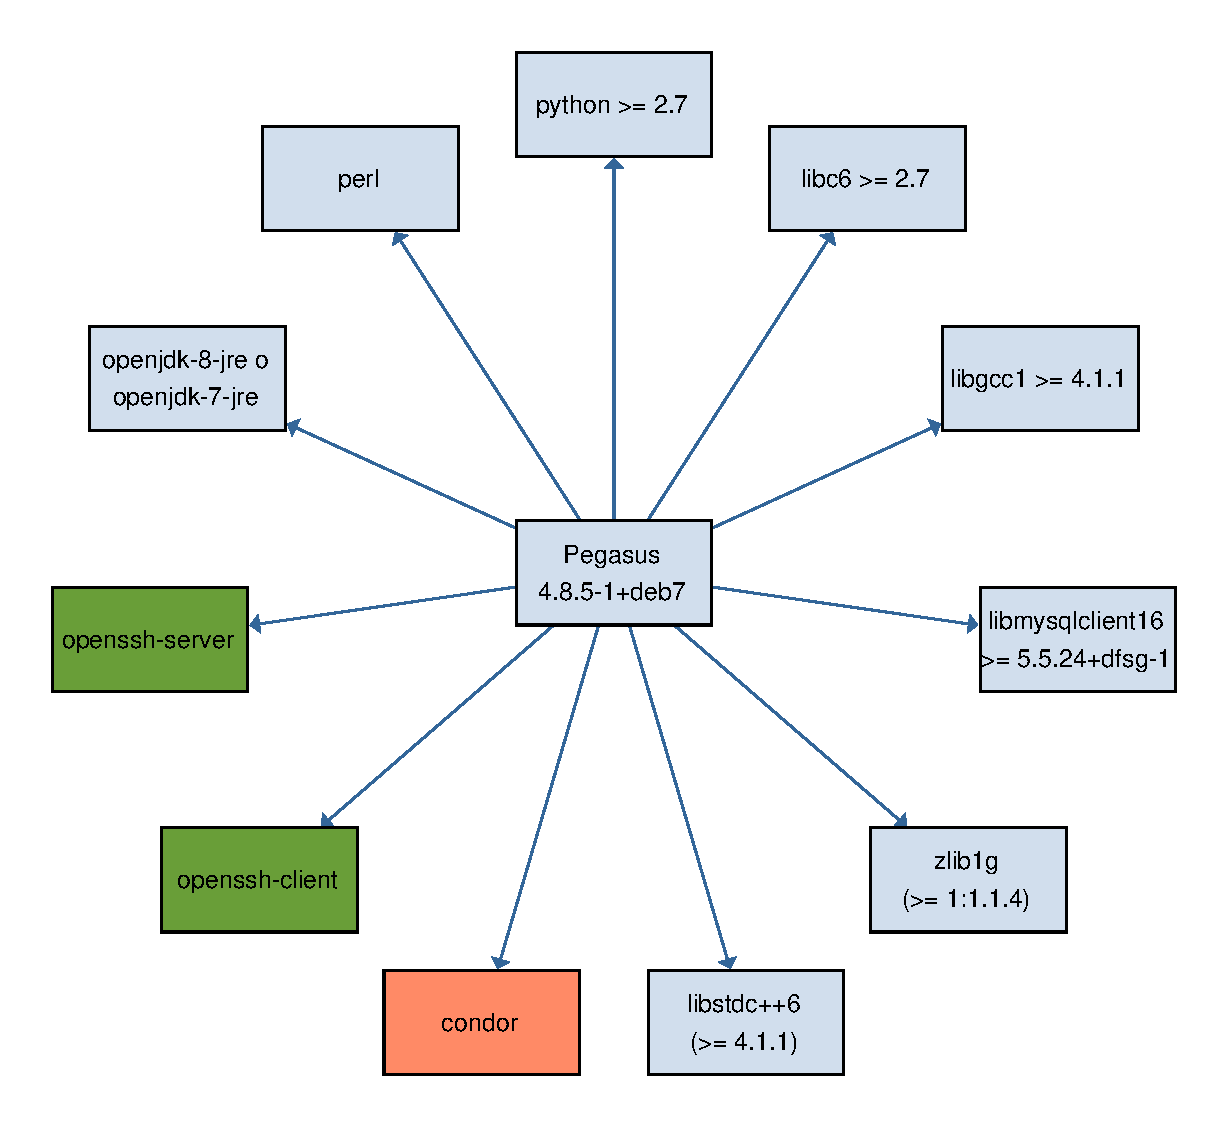
\includegraphics[width=1\textwidth]{Figures/pegasus-deps}
\caption[Dependencias Pegasus]{Dependencias de Pegasus. En gris: dependencias especificadas en el sistema de paquetes. En amarillo: necesarias pero no especificadas en el sistema de paquetes. En verde: dependencias recomendadas}
\label{fig:pegasus-deps}
\end{figure}

Las imágenes se encuentran disponibles en DockerHub~\footnote{\url{https://hub.docker.com/r/dockerpedia/pegasus_workflow_images/}}

\subsubsection{Soybean Knowledge Base}

El workflow SoyKB (Soybean Knowledge Base) \cite{joshi2012soybean} permite realizar un proceso de re-secuencia de germoplasma de la soya, con el objetivo de estudiar rasgos como aceites, proteína, resistencia de los nematodos del quiste de la soya y resistencia al estrés.
Pegasus entrega el workflow y implementa tres operaciones: polimorfismo de nucleótido único (SNP), la operación insertar/remover (indel) de la base del genoma del organismo y una análisis utilizando el software GATK \footnote{\url{https://software.broadinstitute.org/gatk/}}
La figura \ref{fig:soykb} muestra una representación gráfica del workflow, donde se realiza un análisis en paralelo de las muestras. Primero son alineadas con el genoma de referencia,  se identifica los indels y SNPs y luego se fusiona y filtra los resultados. 

\begin{figure}[t]
\centering
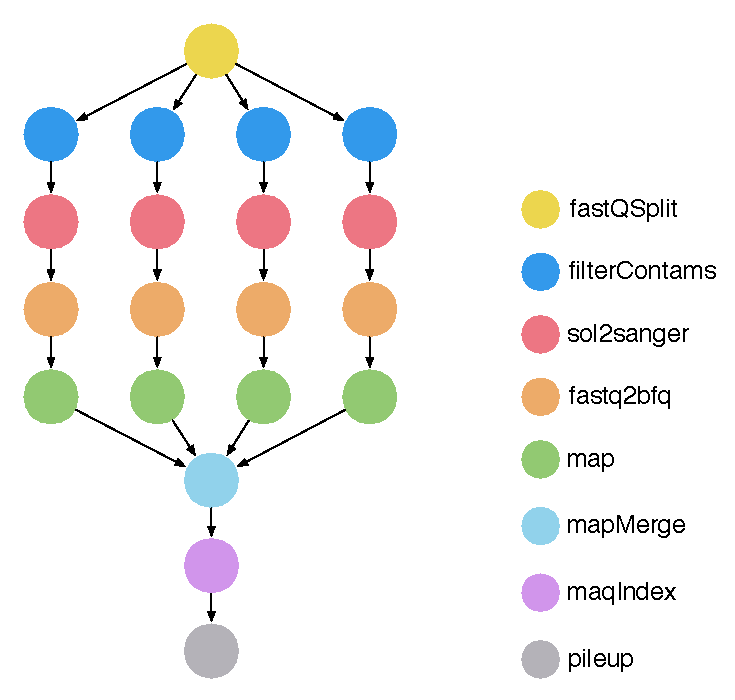
\includegraphics[width=.5\textwidth]{Figures/workflow-genome}
\caption[Representación workflow: SoyKb]{Representación entregada por Pegasus del workflow SoyKB.}\label{fig:soykb}
\end{figure}

Al estudiar la documentación de workflow SoyKB, se han obtenidos los componentes de software expuestos en la figura \ref{fig:soykb-deps}. Esto se clasifican en dos tipos: propio (en amarillo) y de terceros (en verde). Los componentes principales son: bwa, gatk y picard y el software de tercero java sin información dela versión
\begin{figure}[h]
\centering
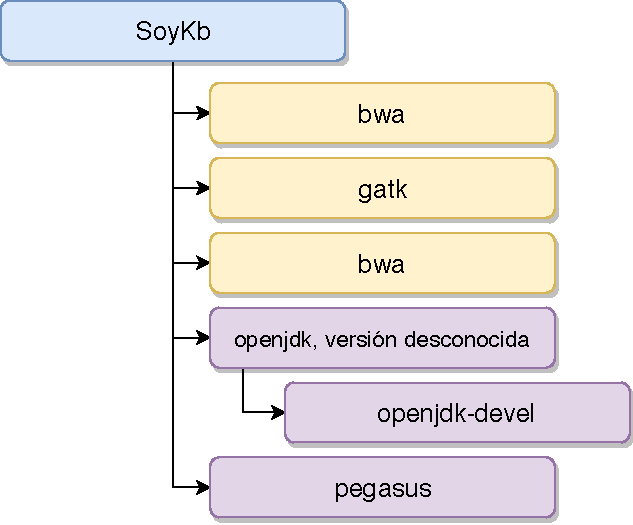
\includegraphics[width=.5\textwidth]{Figures/soykb-deps}
\caption[Dependencias workflow SoyKb]{Dependencias de SoyKb. En amarillo: software propio y en verde software de terceros}\label{fig:soykb-deps} 
\end{figure}

La evaluación de los resultados se realizó de forma manual al igual que en \cite{santana2017reproducibility} debido a los pasos aleatorios del workflow. La metodología de la verificación fue la revisión de la estructura de los resultados, el tamaño de los archivos, número de líneas y la inexistencia de errores. 
Dentro de los resultados se encontraron archivos del tipo VCF que es un formato de archivo de texto que contiene líneas y cada una de las cuales contiene información sobre una posición en el genoma. Según documentación de Pegasus estos son archivos de salida del workflow~\footnote{\url{https://github.com/pegasus-isi/PGen-GenomicVariations-Workflow}}.
Por lo tanto, se realizo una comparación de los archivos y estos no tuvieron diferencias
La imagen se encuentran disponibles en DockerHub ~\cite{soykb-image} y los resultados se encuentran disponibles en ~\cite{soykb-results}

\subsubsection{Montage}

Montage es un conjunto de herramientas creadas por \textit{NASA Infrared Processing and Analysis Center (IPAC)} permitiendo generar bajo demanda mosaicos de imágenes astronómicas personalizadas, se utilizan archivos de entrada que cumplen con el estándar del Sistema de Transporte Flexible de Imágenes (FITS) y que contienen datos de imágenes registrados en proyecciones que cumplen con los estándares del Sistema Mundial de Coordenadas (WCS).

La figura \ref{fig:montage} entregada por Pegasus ilustra el workflow Montage. Cada uno de los nodos de la figura es un software binario que generan la imagen final.

Debido a que el software es un binario, no se encuentra empaquetado. Por lo tanto fue descargado desde la fuente. Las direcciones de descargas se encuentran en el archivo de DockerFile~\cite{montage-image}


\begin{figure}[t]
\centering
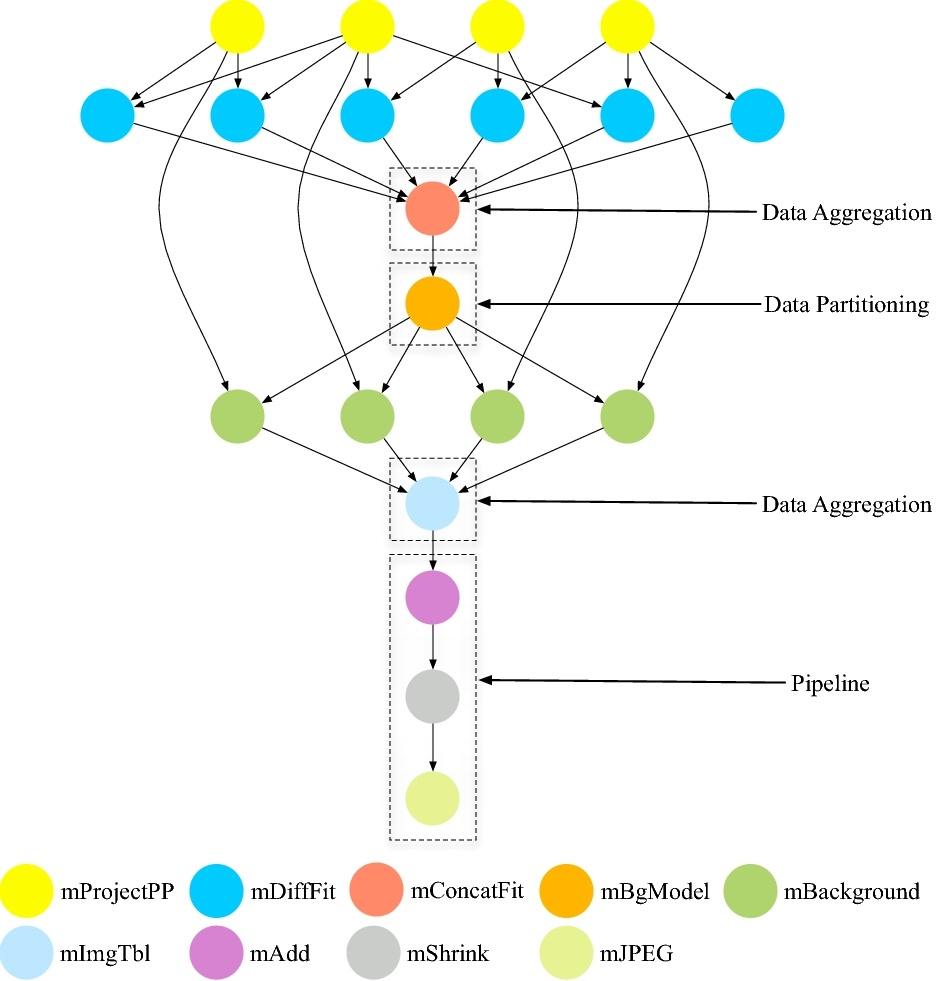
\includegraphics[width=.5\textwidth]{Figures/montage}
\caption[Representación workflow: Montage]{Representación entregada por Pegasus del workflow Montage. Cada uno de los nodos es una operación y la leyenda indica el nombre de la operación.}\label{fig:montage}
\end{figure}

Dado que los resultados de Montage son imágenes, se utiliza la herramienta de hash perceptual \footnote{\url{http://phash.org}} para realizar la comparación entre la imagen reproducida (imagen del cielo de 0,1 grados) frente a la original.
Como resultado, se obtiene un factor de similitud de 1,0 (de 1,0).
Las figuras \ref{fig:montage-wicus} y \ref{fig:montage-mosorio} muestran las imágenes resultantes y los archivos resultantes en formato FITS se encuentran en el repositorio ~\cite{montage-results}. 
La imagen se encuentran disponibles en DockerHub ~\cite{montage-image}

\begin{figure*}[t]
    \centering
    \begin{subfigure}[b]{0.4\textwidth}
         \centering
         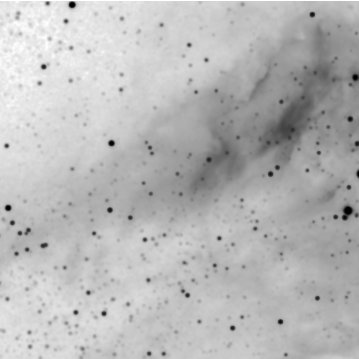
\includegraphics[width=\textwidth]{Figures/montage-original}
         \caption[Resultados workflow original: Montage]{Resultados originales obtenidos desde WICUS}
         \label{fig:montage-wicus}
     \end{subfigure}
         ~ 
	    \begin{subfigure}[b]{0.4\textwidth}
         \centering
         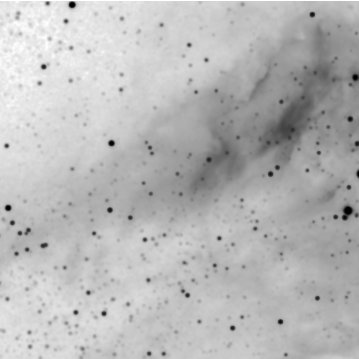
\includegraphics[width=\textwidth]{Figures/montage-mosorio}
         \caption[Resultados workflow reproducidos: Montage]{Resultados reproducidos por nuestra propuesta}
         \label{fig:montage-mosorio}
     \end{subfigure}
        \caption[Comparación resultados Montage]{Los resultados obtenidos con el nuevo ambiente son iguales}
        \label{fig:montage-results}
\end{figure*}


\subsection{dispel4py}

dispel4py~\cite{DBLP:conf/eScience/FilgueiraKAKSS15} es una biblioteca Python para describir workflow para aplicaciones intensivas de datos, que luego se traducen y ejecutan en plataformas distribuidas (por ejemplo, Apache Storm, clusters MPI, etc.).
El paquete dispel4py ha sido obtenido del repositorio oficial \footnote{\url{https://github.com/rosafilgueira/dispel4py_workflows}}. 
Para la instalación el paquete, se utiliza Conda, un gestor de paquetes, dependencias y entornos para lenguajes Python, R, Ruby, Lua, Scala, Java, JavaScript, C/ C++, FORTRAN y que es ampliamente utilizado en entornos de \textit{Jupyter notebook}. 
Los principales requisitos de dispel4py obtenidos de la documentación son: Python2.7, git y  Python-setuptools
Las imágenes se encuentran disponibles en DockerHub~\footnote{\url{https://hub.docker.com/r/dockerpedia//}}



\subsubsection{Internal extinction}

\textit{Internal Extinction of Galaxies} workflow calcula la extinción interna de galaxias desde el catalogo Amiga. Estos datos son obtenidos a partir de un servicio llamado Observatorio Virtual, que es una red de herramientas y servicios que implementan estándares publicados por la \textit{International Virtual Observatory Alliance} (IVOA). El workflow calcula una propiedad, que representa la extinción de polvo dentro de las galaxias y que es un coeficiente de corrección necesario para calcular la luminosidad óptica de una galaxia.

El workflow primero lee el archivo de inicio que contiene la declinación y ascensión recta de 1051 galaxias. Luego, utiliza estos valores para realizar consultas al observatorio virtual. Los valores resultantes de las consultas son filtrados y se seleccionan sólo los valores que correspondan al tipo morfológico (Mtype) y al rango de los ejes del isófito 25 $mag/arcsec^{2}$ (logr25) de las galaxias. Finalmente, se calcula su extinción interna. La figura \ref{fig:internal} muestra los pasos del workflow

\begin{figure}[t]
\centering
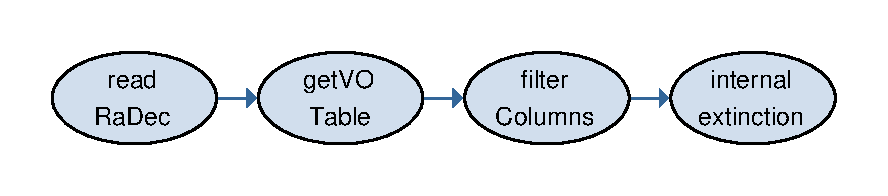
\includegraphics[width=.8\textwidth]{Figures/internal-extinction}
\caption[Representación workflow: Internal Extinction]{Pasos necesarios para el workflow Internal Extinction}\label{fig:internal}
\end{figure}

Nuestra investigación inicial sobre las dependencias para la ejecución de Internal extinction muestra que el software principal requeridos es el siguiente:  \verb|requests|, \verb|python=|, \verb|numpy| y \verb|astropy|


\todo{comparar}
La imagen se encuentran disponibles en DockerHub ~\cite{internal-image} y los resultados se encuentran disponibles en ~\cite{internal-results}


\subsubsection{Seismic Ambient Noise Cross-Correlation}
\textit{Seismic Ambient Noise Cross-Correlation workflow} (o xcorr workflow) es parte del proyecto \textit{Virtual Earthquake and seismology Research Community e-science environment in Europe} (VERCE). 
El objetivo del workflow es la previsión de riesgos producidos por terremotos y erupciones volcánicas. Estos eventos en ciertos casos van precedidos o acompañados de cambios en las propiedades geofísicas de la Tierra, como la velocidad de las olas.
Para lograr desarrollo de métodos fiables de evaluación de riesgos para estas amenazas se requiere un análisis en tiempo real de los datos sísmicos y un pronóstico verdaderamente prospectivo y pruebas para reducir los sesgos.

\texttt{xcorr} logra lo anterior a través de dos etapas, la primera etapa es un pre-procesamiento de series de tiempo de una estación sísmica llamadas trazas, en esta etapa se realiza una serie de tratamientos y el procesamiento de cada traza que es independiente de las otras, haciendo que esta fase sea paralela. 
Luego la segunda etapa se empareja todas las estaciones y calcula la correlación cruzada para cada par. La figura \ref{fig:xcorr} muestra los pasos del workflow.


\begin{figure}[t]
\centering
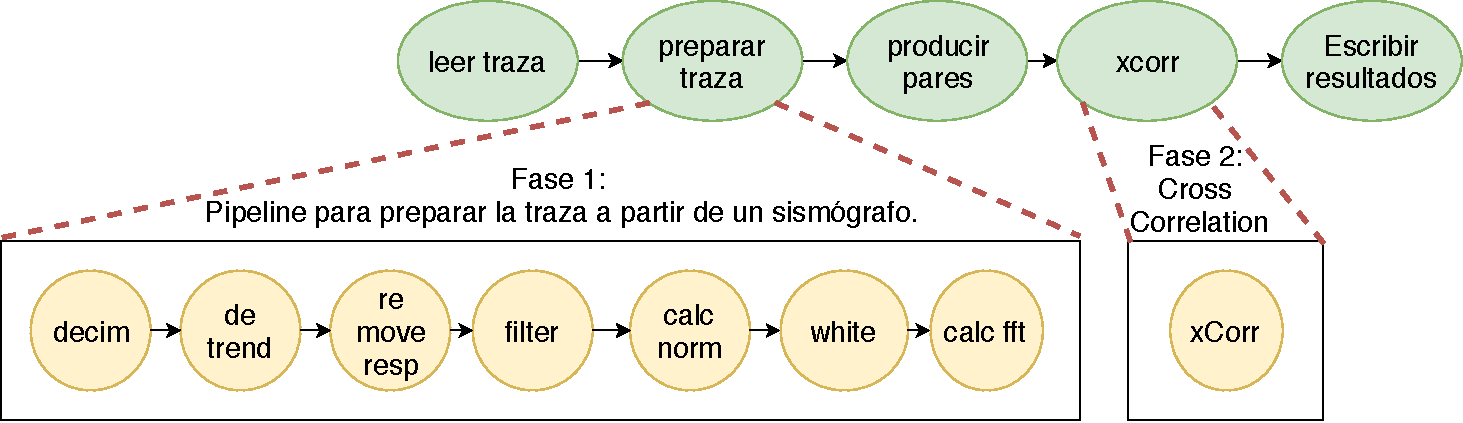
\includegraphics[width=.8\textwidth]{Figures/xcorr}
\caption[Representación workflow: Seismic Ambient Noise Cross-Correlation]{Representación workflow: Seismic Ambient Noise Cross-Correlation}\label{fig:xcorr}
\end{figure}


Nuestra investigación inicial sobre las dependencias para la ejecución indica que los componentes de software necesarios son: \verb|python|, \verb|obspy| y \verb|numpy|

Respecto a los resultados, las ejecuciones en máquina virtual y contenedores obtuvieron el mismo resultado. 

La imagen se encuentra disponible en DockerHub~\cite{xcorr-image} y los resultados en GitHub~\cite{xcorr-results}.

\subsection{WINGS}

WINGS~\cite{DBLP:journals/expert/GilRKGGMD11} es un sistema de flujo de trabajo semántico que ayuda a los científicos en el diseño de experimentos computacionales. 
En WINGS, se especifica cómo deben ser procesados los conjuntos de datos por una serie de componentes en una configuración particular.
WINGS a diferencia de los otros sistemas de workflows utiliza imágenes Docker para su distribución. Pese a que WINGS presenta las imágenes de Docker, estas imágenes son una caja negra y no es posible obtener los componentes de software.
La investigación inicial sobre las dependencias indica que los principales requisitos de WINGS son: Java 1.8, Tomcat 8.5, Docker. La figura \ref{fig:wings-deps} muestra en mayor detalles las dependencias especificadas tanto por el sistema de paquetes o documentación.

\begin{figure}[t]
\centering
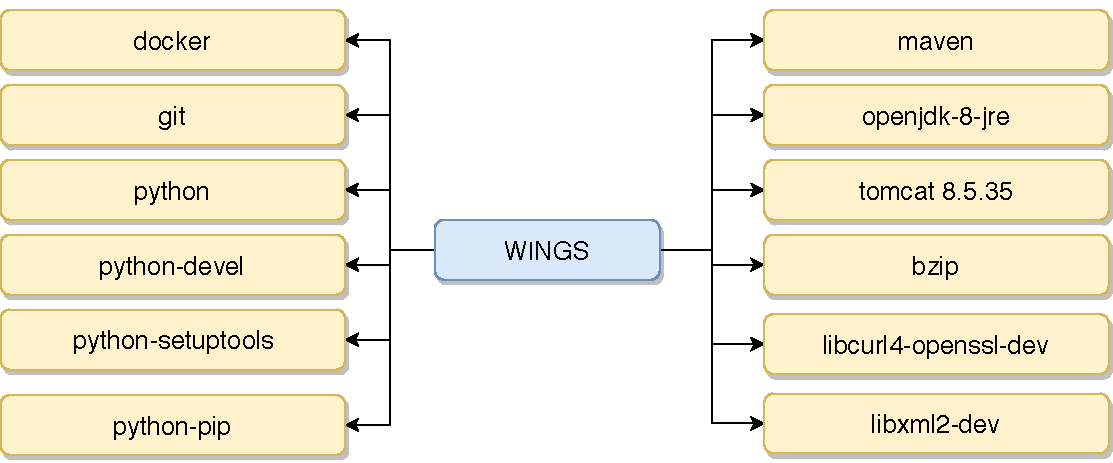
\includegraphics[width=.8\textwidth]{Figures/wings-deps}
\caption{Dependencias de WINGS}\label{fig:wings-deps}
\end{figure}


\subsubsection{MODFLOW-NWT}

MODFLOW es el modelo hidrológico modular del \textit{United States Geological Survey}~\footnote{\url{https://www.usgs.gov}} (USGS). MODFLOW se considera una norma internacional para simular y predecir las condiciones de las aguas subterráneas y las interacciones entre las aguas subterráneas y superficiales.
El USGS MODFLOW-NWT es una formulación de Newton-Raphson para MODFLOW-2005 con el objetivo de mejorar la solución de problemas de flujo, secado y humectación de aguas subterráneas no confinadas.

\begin{figure}[t]
\centering
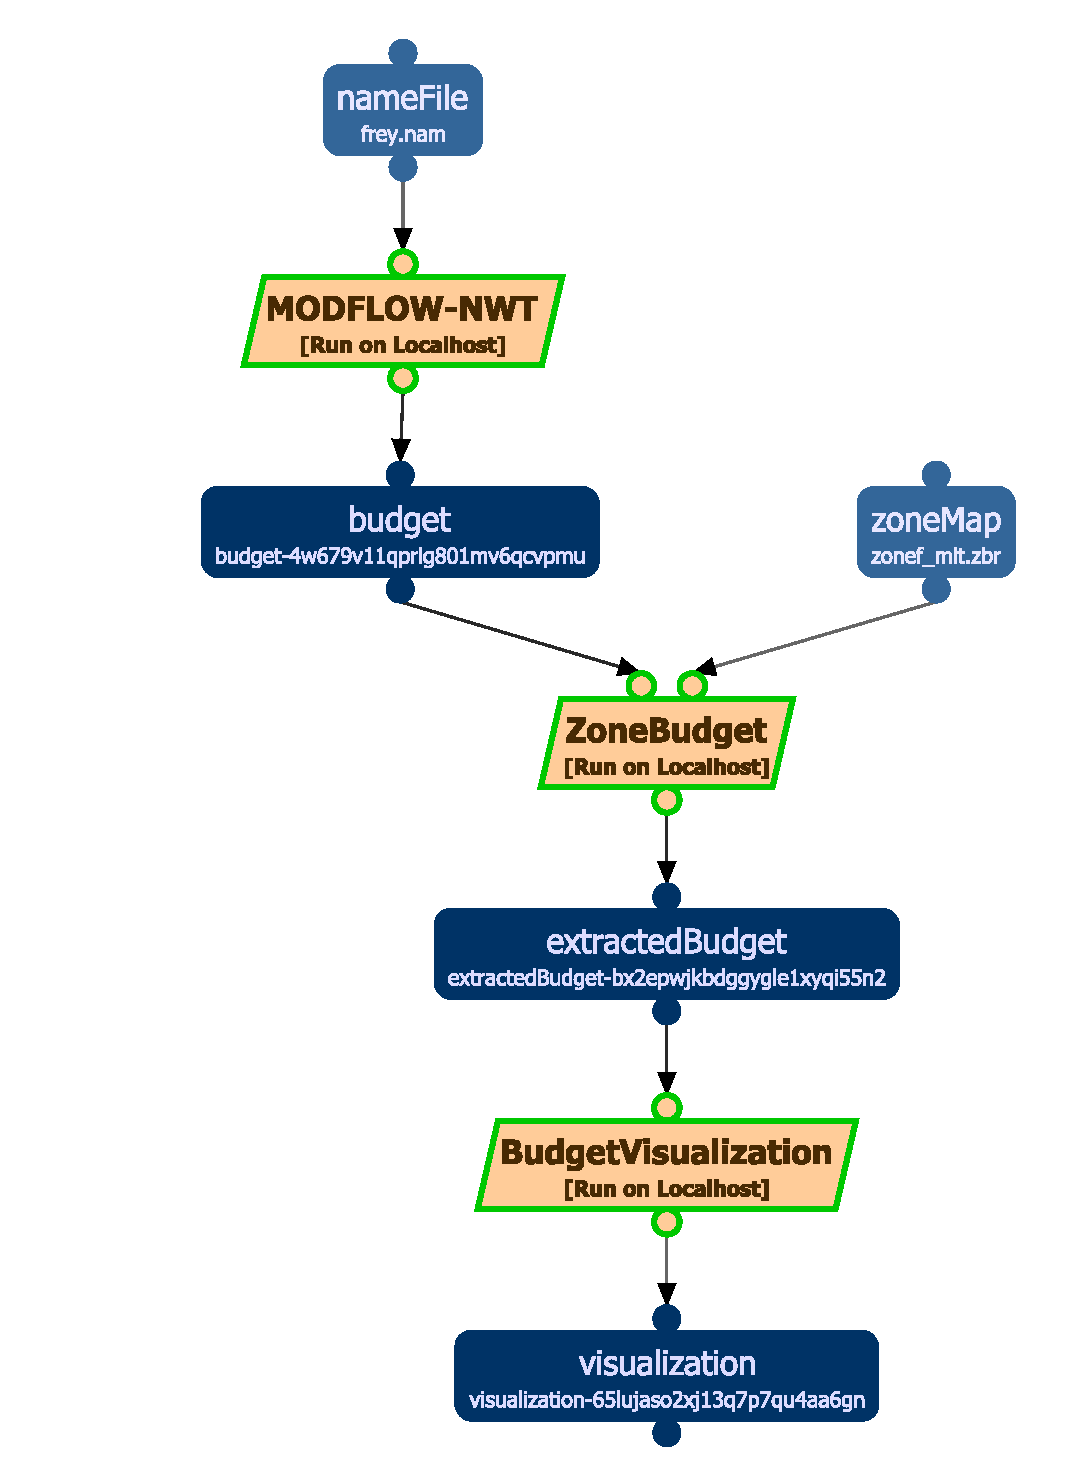
\includegraphics[width=0.6\textwidth]{Figures/usgs-modflow-nwt}
\caption{Representación workflow: MODFLOW-NWT}
\label{fig:modflow}
\end{figure}


La figura \ref{fig:modflow} muestra la estructura principal del workflow, desarrollado como un workflow compuesto por tres pasos. El proceso inicia leyendo el modelo a utilizar. Luego, el archivo de zona se usa para especificar arreglos que van usarse y finalmente se genera una visualización que muestra la cantidad de millones de galones por día en zona. Las figuras \ref{fig:modflow-original} y \ref{fig:modflow-reproduced} muestran los resultados generados por el ambiente original y reproducido respectivamente.

\begin{figure*}[t]
    \centering
    \begin{subfigure}[b]{\textwidth}
         \centering
         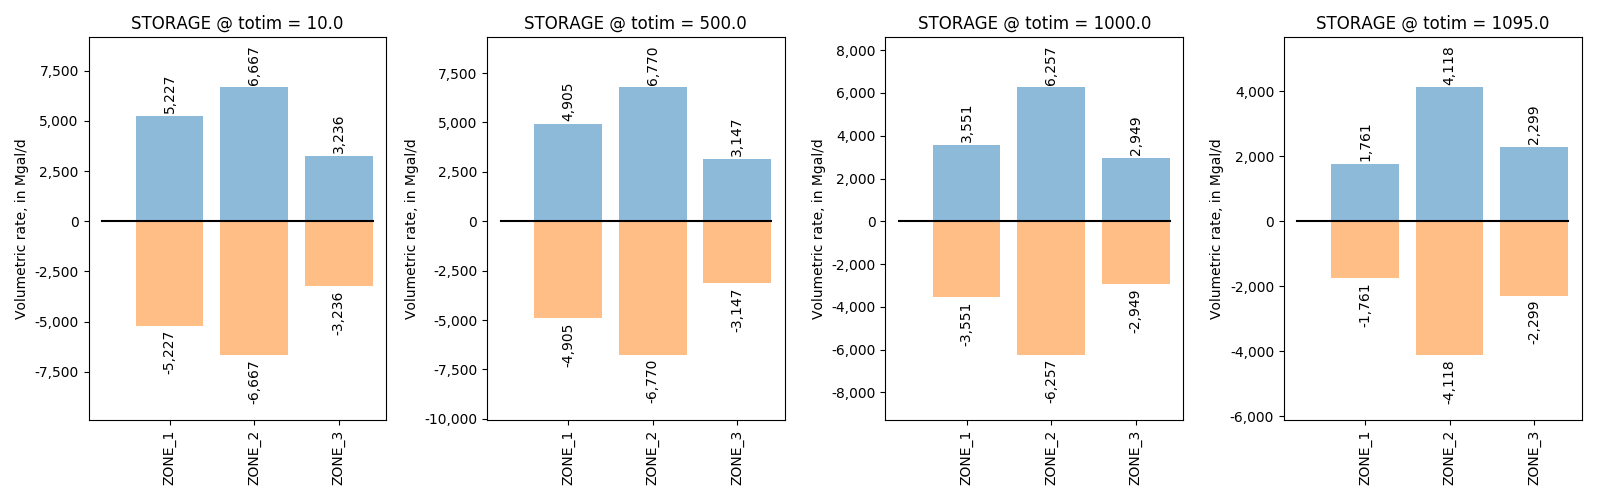
\includegraphics[width=\textwidth]{Figures/viz-original}
         \caption[Resultados workflow originales: ModFlow]{Resultados originales entregados por el Information Sciences Institute}
         \label{fig:modflow-original}
     \end{subfigure}
	
	    \begin{subfigure}[b]{\textwidth}
         \centering
         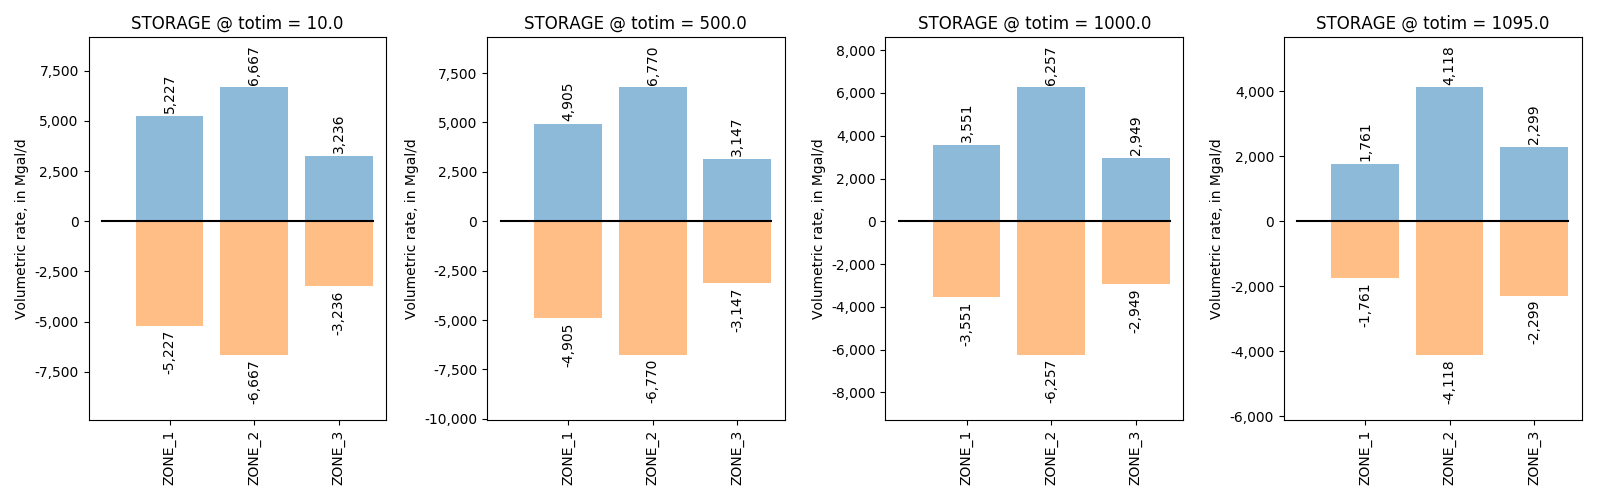
\includegraphics[width=\textwidth]{Figures/viz-reproduced}
        \caption[Resultados workflow reproducidos: ModFlow]{Resultados reproducidos por nuestra propuesta}
         \label{fig:modflow-reproduced}
     \end{subfigure}
        \caption[Comparación resultados MODFLOW-NEW]{Los resultados obtenidos son idénticos}
        \label{fig:both-modflow}
\end{figure*}






%-----------------------------------------------
% 5.2 Physical conservation
%-----------------------------------------------
\section{Conservación física}\label{s5.2}

Todas las imágenes son publicadas con su correspondiente Dockerfile y cualquier usuario puede inspeccionarlas y mejorarlas. Las imágenes puede ser encontradas en DockerHub \footnote{https://hub.docker.com/u/dockerpedia/}\cite{xcorr-image,internal-image,soykb-image,montage-image,wings-image}  y GitHub \footnote{\url{https://github.com/dockerpedia}} \cite{xcorr-results,internal-results,soykb-results,montage-results,wings-results}. 

Para evaluar la reproducibilidad del ambiente computacional se utiliza tres proveedores diferentes: DigitalOcean, Google Cloud y un local. La figura de \ref{image-env} presenta una descripción de las características de los ambientes    

\begin{table}[t]
\centering
\begin{tabular}{|l|l|l|l|}
\hline
Resource   & Digital Ocean & Google Compute & Local     \\ \hline
RAM (GB)   & 8             & 8              & 4         \\ \hline
Disk (GB)  & 100           & 100            & 70        \\ \hline
CPU (GHz)  & 2.0           & 2.5            & 2.8          \\ \hline
CPU (Cores)& 4             & 2              & 4          \\ \hline
CPU (Arch) & 64            & 64             & 64        \\ \hline
OS         & Centos 7      & Debian 9       & Fedora 27 \\ \hline
\end{tabular}
\caption{Características de hardware de pruebas.}
\label{image-env}
\end{table}

El ambiente debe tener instalado Docker, cada imagen en su manifiesto describe la versión de Docker con cuál fue construida. Sin embargo, Docker asegura idempontencia para los ambientes CentOS7, Debian 10/9/8/7.7, Fedora 26/27/28, Ubuntu 14.04/16.06/18.04, Windows 10, macOS El Capitan 10.11 o nuevas versiones.
El proceso de instalación puede ser encontrado en la documentación oficial \footnote{\url{https://docs.docker.com/install/}}.

Cada imagen de Docker tiene archivo README con las instrucciones para correr el experimento. Las figuras \ref{lst:1}~\ref{lst:2} y~\ref{lst:3}  muestran los pasos necesarios para correr el experimento computacional: SoyKB. 

El primer paso es correr el experimento y descargar la imagen:
\begin{figure*}[ht]
\begin{lstlisting}[caption={Descargar y correr la imagen disponible en DockerHub mosorio/pegasus\_workflow\_images:soykb},label={lst:1},language=bash]
docker run -d --rm -it --name soybean \
 mosorio/pegasus_workflow_images:soykb
\end{lstlisting}	
\end{figure*}


Luego, el usuario debe entrar al container. El usuario puede confirmar que se encuentra dentro del container por el cambio de símbolo de la terminal  (prompt).
\begin{figure*}[ht]
\begin{lstlisting}[caption={Entrar al ambiente computacional utilizando bash},label={lst:2},language=bash]
root@docker-instance:~# docker exec \
-ti -u workflow:workflow soybean bash
workflow@a0f861e6fbc4:~ 
\end{lstlisting}
\end{figure*}

Finalmente, correr el workflow. 

\begin{figure*}[ht]
\begin{lstlisting}[caption={Run the workflow},label={lst:3},language=bash]
workflow@a0f861e6fbc4:~/soykb \
./workflow-generator --exec-env distributed	
\end{lstlisting}
\end{figure*}

Para evaluar si las imágenes Docker son livianas y almacenables, se construyeron dos imágenes, una utilizando Docker y otra utilizando máquinas virtuales. La imagen de Docker se construyó bajo nuestro enfoque y la imagen de la máquina virtual basada en el trabajo de ~\cite{santana2017reproducibility}. Luego se compara el uso de disco de ambas.

%-------------------------------------------
% Logical conservation
%-----------------------------------------------
\section{Conservación lógica}\label{s5.3}

A través de las anotaciones realizadas, se busca describir los ambientes computacionales en forma automática, comparar las diferencias entre dos ambientes y construir un ambiente computacional similar que permita la ejecución del workflow. 

Para ello, se anota de manera automática los workflows con nuestra herramienta, las anotaciones están agrupadas por: pasos de construcción y componentes de software. 

Para evaluar la calidad de las anotaciones se utilizan dos experimentos.

\begin{itemize}
	\item Reproducir el ambiente utilizando los pasos de construcción representados por DeploymentPlan.
	\item Detectar las similitudes y diferencias entre dos ambientes computacionales.
\end{itemize}

Para obtener las anotaciones, se propone e implementa usar Clair y construir un sistema de anotador. La figura \ref{fig:arch} muestra los pasos principales del sistema.

\begin{figure*}[t]
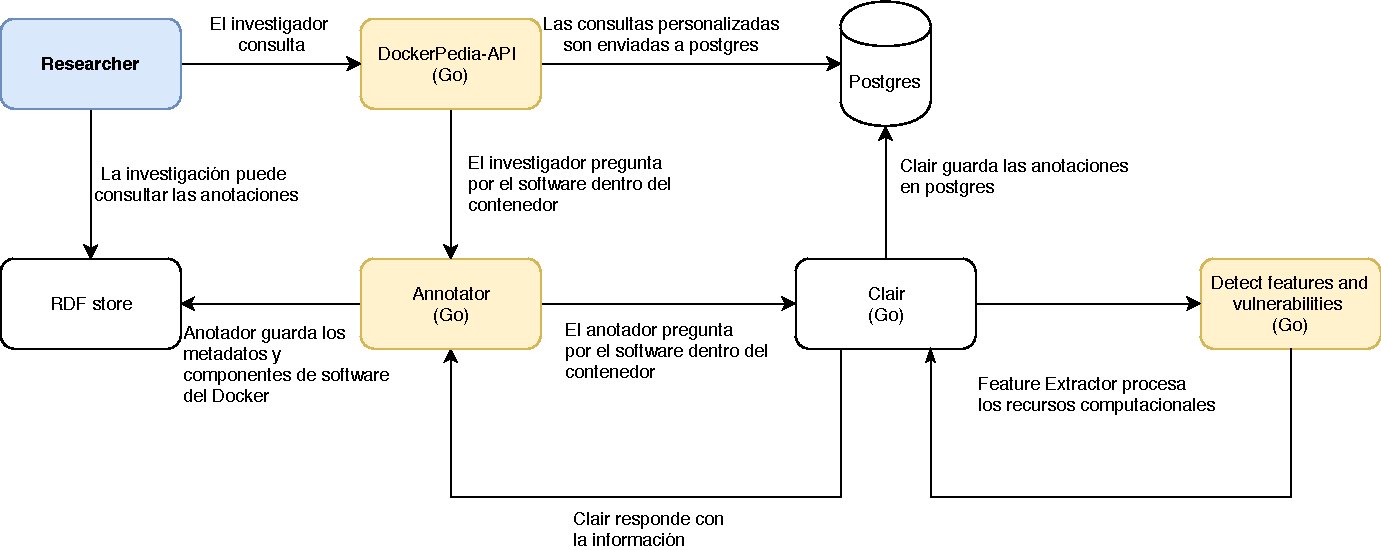
\includegraphics[width=\textwidth]{Figures/arch.pdf}
\caption[Arquitectura sistema anotador]{El sistema anotador permite recibir la información de la imagen, consultar los componentes de software a nuestra versión de Clair, obtener metadatos desde el manifesto y almacenar la información en forma de triples en Apache Jena.}\label{fig:arch}
\end{figure*}


\begin{enumerate}
    \item El investigador pregunta sobre la información de una imagen al sistema anotador. El sistema anotador se encuentra escrito en GoLang y disponible en nuestro repositorio.
    \item El sistema anotador pregunta a Clair sobre software y sus vulnerabilidades de la imagen. El sistema de Clair es una versión propia que puede detectar componentes de software instalado por Conda.
    \item Para obtener los pasos de construcción, etiquetas, arquitectura y más información. El anotador obtiene el manifiesto de la imagen desde DockerHub
    \item El sistema anotador guarda la información usando RDF y la ontología propuesta.
\end{enumerate}


Para reproducir el entorno, el sistema obtiene el repositorio asociado a la imagen y construye la nueva imagen. La URL del repositorio y el cambio asociado (representado por un VCS commit) se pueden obtener por dos métodos: consultando nuestras anotaciones o usando un comando Docker. El listado \ref{lst:inspect_command} muestra las etiquetas de la imagen de flujo de trabajo SoyKB.

\begin{figure*}[h]
\begin{lstlisting}[caption={Inspeccionar las anotaciones de una imagen},label={lst:inspect_command},language=bash]
root@docker-instance:~# docker inspect \ 
    --format='{{json .Config.Labels}}' \ 
    dockerpedia/soykb:latest
\end{lstlisting}
\end{figure*}

La figura \ref{lst:inspect_result} muestra algunas de las etiquetas de la imagen basado en \textit{Open Container Initiative}. Y todas las imágenes disponibles en nuestros repositorios presentan esas etiquetas.

\begin{figure*}
\begin{lstlisting}[caption={Inspect image annotations},label={lst:inspect_result},language=json]
{
"maintainer": "Maximiliano Osorio <mosorio@inf.utfsm.cl>",
"org.label-schema.build-date": "2018-11-10T21:11:28Z",
"org.label-schema.name": "Soybean Knowledge Base",
"org.label-schema.schema-version": "1.0",
"org.label-schema.url": "http://www.soykb.org/",
"org.label-schema.vcs-ref": "15955b0",
"org.label-schema.vcs-url": "https://github.com/dockerpedia/soykb",
"org.label-schema.vendor": "DockerPedia",
"org.label-schema.version": "1.0"
}

\end{lstlisting}
\end{figure*}

Para evaluar si los entornos son similares, comparamos ambas imágenes utilizando el lenguaje de consulta SPARQL 1.1. El experimento fue un caso real que permitió detectar un problema en la ejecución del workflow SoyKB 
La figura \ref{lst:compare_query} muestra la consulta para identificar los componentes diferentes de software entre dos imágenes y la figura \ref{lst:compare_query_2} muestra muestra la consulta para identificar los componentes iguales de software entre dos imágenes.
\begin{figure*}
\begin{lstlisting}[caption={¿Cuáles son los diferentes componentes entre dos imágenes?},label={lst:compare_query},language=sparql]
SELECT * WHERE {
 pegasus_workflow_images%3Alatest
  vocab:containsSoftware ?p .
 MINUS{
 pegasus_workflow_images%3Apegasus-4.8.5
  vocab:containsSoftware ?p   
 }
}
\end{lstlisting}
\end{figure*}

\begin{figure*}

\begin{lstlisting}[caption={¿Cuáles son los componentes que comparten entre dos imágenes?},label={lst:compare_query_2},language=sparql]
SELECT * WHERE {
 pegasus_workflow_images%3Alatest
      vocab:containsSoftware ?p .
 pegasus_workflow_images%3Apegasus-4.8.5
      vocab:containsSoftware ?p   
    }
    \end{lstlisting}
    \end{figure*}

    
\section{Resultados y discusión}\label{s5.4}
Se logró ejecutar los workflows utilizando imágenes Docker sobre sus plataformas correspondientes.
Sin embargo, no fue un tarea simple. La información de los componentes de software para los cincos workflows no se encontraba disponible o era incompleta. Por lo que encontrar los componentes necesarios para construir la imagen fue una tarea forense, donde se tuvo que realizar múltiples ejecuciones con distintos componentes de software hasta lograr la ejecución. 
Lo cual no es una tarea trivial inclusive para expertos de área de las ciencias de la computación.
Todas las ejecuciones se compararon con la imagen VM predefinida, donde ya existía un entorno de ejecución. Los resultados muestran que los ambientes de ejecución de contenedores son capaces de ejecutar completamente sus workflow relacionados. Se  comprobó que no sólo los workflows se ejecutan con éxito, sino también que los resultados son correctos y equivalentes a través de los datos de salida producidos. 

Por otra parte, los resultados experimentales muestran que nuestra propuesta puede detectar automáticamente los componentes del software, las vulnerabilidades relacionadas, los pasos de construcción y los metadatos específicos de los experimentos científicos en forma de imágenes Docker. 
Además, los resultados muestran que es posible extender Clair para anotar a otros gestores de paquetes. 

Aún mas, las anotaciones generadas por nuestro enfoque permiten comparar los componentes de software entre dos o más entornos. Esta función se puede utilizar como herramienta de depuración cuando un entorno reproducido no funciona.
Por ejemplo, en agosto de 2018, se construyó la imagen del workflow SoyKB, y se pudo ejecutar el workflow con éxito. Sin embargo, se reconstruyó una nueva imagen en noviembre con el mismo DeploymentPlan y no se pudo ejecutar el workflow con éxito.


Se utilizaron las anotaciones de los componentes de software dentro de ambas imágenes. Y se encontró las siguientes diferencias:
\begin{itemize}
    \item Agosto: Pegasus 4.8 y Java 1.7
    \item Noviembre: Pegasus 4.9 y Java 1.8
\end{itemize}

Luego se analizó el código y la documentación de SoyKB y las dependencias de Pegasus 4.9. Como resultado, sé obtuvo las gráficas de dependencia mostradas en la figura \ref{fig:pegasus49}.  Los gráficos de dependencia muestran que el paquete Pegasus 4.9 y SoyKB no son compatibles debido a sus requerimientos de versión Java.

Y construyó una nueva imagen instalando Pegasus 4.8, y se obtuvo los gráficos de dependencia que se muestran en la figura \ref{fig:pegasus48}. Aquí, el gráfico no tiene un conflicto y se pudo ejecutar el workflow con éxito.

La nueva imagen fue nombrada como: \verb|pegasus_workflow_images:4.8.5|


\begin{figure*}[t]
    \centering
    \begin{subfigure}[b]{0.40\textwidth}
         \centering
         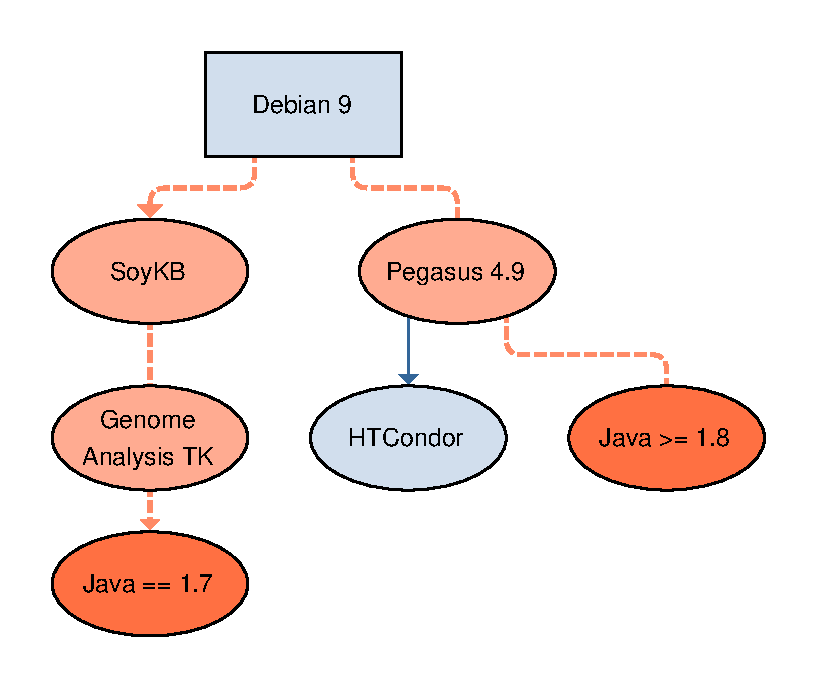
\includegraphics[width=\textwidth]{Figures/pegasus-49.pdf}
         \caption{Gráfico de dependencias Pegasus 4.9 y SoyKB}
         \label{fig:pegasus49}
     \end{subfigure}
    ~ 
    \begin{subfigure}[b]{0.40\textwidth}
         \centering
         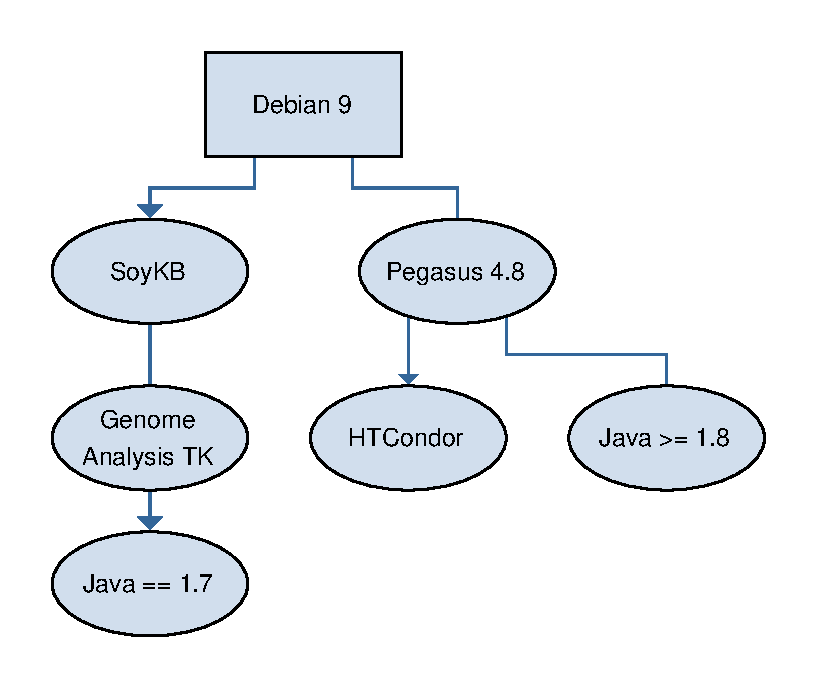
\includegraphics[width=\textwidth]{Figures/pegasus-48.pdf}
         \caption{Gráfico de dependencias Pegasus 4.8 y SoyKB}
         \label{fig:pegasus48}
     \end{subfigure}
        \caption{Análisis de dependencias imágenes Pegasus}
        \label{fig:dependencies-graph}
\end{figure*}

Considerando que la razón principal de los trabajos anteriores para evitar la conservación física era la gran demanda de almacenamiento de máquinas virtuales. Se realizó una comparación  del uso del disco, los resultados muestran una disminución del 64,2\% para la imagen Pegasus y del 41,5\% para la dispel4py. La tabla \ref{storage-reduce} muestra la diferencia para el sistema de flujo de trabajo Pegasus y dispel4py.

\begin{table}[t]
\centering
\begin{tabular}{|l|l|l|}
\hline
Enfoque        & Pegasus (MB) & dispel4py (MB) \\ \hline
Virtualization & 1929         & 3509 \\ \hline
Container      & 690          & 2500 \\ \hline
\end{tabular}
\caption[Comparación de uso de disco entre VMs y contenedores]{Uso de disco de las imágenes pegasus y dispel4py utilizando máquinas virtuales y contenedores}
\label{storage-reduce}
\end{table}


En este capítulo se ha introducido cada uno de los WMSs y workflows correspondientes y se ha descrito el proceso de creación de las imágenes para uno de ellos.
Luego, se expone que es posible describir los componentes de software y pasos de los construcción y utilizar esas descripciones para reproducir el ambiente computacional requerido. 
Asimismo, se muestran el framework completo propuesto y cómo las anotaciones y los modelos semánticos permiten la resolución un problema real producido por cambios los componentes de software en un ambiente computacional.
 
En el siguiente capítulo se muestra 
\include{Chapters/Chapter6/chapter6}


\bibliographystyle{ieeetr}
\bibliography{References/references}

\end{document}
